\chapter{Towards Optimal Query Term Selection}
\label{cha:analysis}
In this chapter, we will investigate the problem from term analysis perspective for both Patent Query and relevant documents because we are interested 
in finding what is wrong in term matching process between the Patent Query and relevant patents. 
We start with experiments which show sufficient term overlap between the Patent Query and relevant documents, 
then we introduce an Oracular Relevance Feedback scoring criteria to discriminate useful terms from noisy terms. 
We formulate two Oracular Query, based on this score, that give us an upper-bound performance. In addition, our experiments demonstrate the sufficiency of terms in the Patent Query to achieve a high performance. 
We try four simple query reduction approaches and we discuss the reasons that they are not efficient.  
Finally, we show that we can get improved using a simple, minimal feedback interactive approach.
%%%%%%%%%%%%%%%%%%%%%%%%%%%%%%%%%%%%%%%%%%%%%%%%%%%%%%%%%%%%%%
%%%%%%%%%%%%%%%%%%%%%%%% SECTION 1 %%%%%%%%%%%%%%%%%%%%%%%%%%
%%%%%%%%%%%%%%%%%%%%%%%%%%%%%%%%%%%%%%%%%%%%%%%%%%%%%%%%%%%%%%

\section{Term Mismatch}
\label{sec:termmismatch}
%\input{TermAnalysis/termmismatch}
Standard retrieval models rank documents based on term matching between the query and documents.  
A significant term mismatch between the query patent and relevant patents has been mentioned the
main cause for low effective patent prior art search in previous works~\citep{roda2010clef}~\citep{magdy2012toward}. 
We examine term overlap between Patent Query and three different patent documents: (i) retrieved relevant patents (TPs), (ii) retrieved non-relevant patents (FPs), and (iii) non-retrieved relevant patents (FNs), respectively, by calculating the average term overlap per query as follows:
%%%%%%%%%%%%%%%%%%%%%%%%%%%%%%%%%%%%%%%%%%%%%%%%%%%%%%%%%%%%%%
\begin{equation} 
TO (Q) = \frac{1}{|D|}\sum_{d\in D}\frac{|terms_{Q\cap d}|}{|Q|}
\label{eq:fntermoverlap}
\end{equation}
%\vspace*{-1ex}
%\begin{displaymath}t\in \lbrace \mbox{terms in top-100 retrieved documents}\rbrace\end{displaymath}
%%%%%%%%%%%%%%%%%%%%%%%%%%%%%%%%%%%%%%%%%%%%%%%%%%%%%%%%%%%%%%
where $TO(Q)$ is the average term overlap per query --- we calculate this score for TP, FP, and FN patents respectively, $D$ is a collection of TP patents, FP patents, or FN patents for each query respectively, $|D|$ is the number of TP patents, FP patents, or FN patents for each query, $ |terms_{Q\cap d}| $ is the number of query terms appear in each TP, FP, or FN patent, $ |Q| $ is the size of the query.

The results has been illustrated in Figure~\ref{fig:overlap}. We conclude two main facts:
\begin{enumerate}
\item For the majority of queries (around 94\% of queries), patent documents are retrieved (TPs and FPs) when they have a term overlap with a query above $ 0.2 $.
\item We can also see sufficient term overlap with the query for FN patents, whereas, compared to TPs and FPs, more queries can be seen with the term overlap less than $ 0.2 $ (about 24\% of queries). 
\end{enumerate}
 
%%%%%%%%%%%%%%%%%%%%%%%%%%%%%%%%%%%%%%%%%%%%%%%%%%%%%%%%%%%%%%
\begin{figure}[t!]
\begin{centering}
\subfigure[Query and TP patents.]{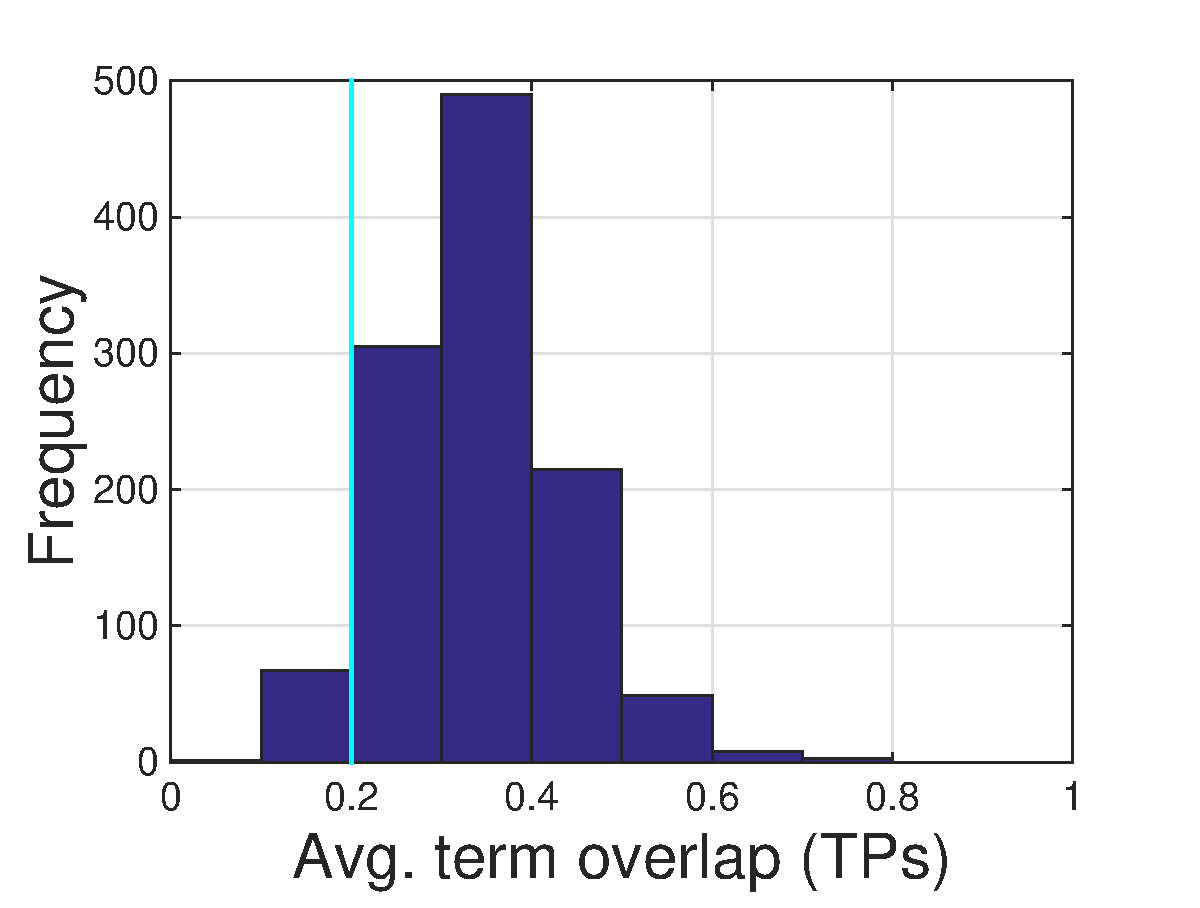
\includegraphics[width=5cm]{figs/to-tps.eps}}\subfigure[Query and FP patents.]{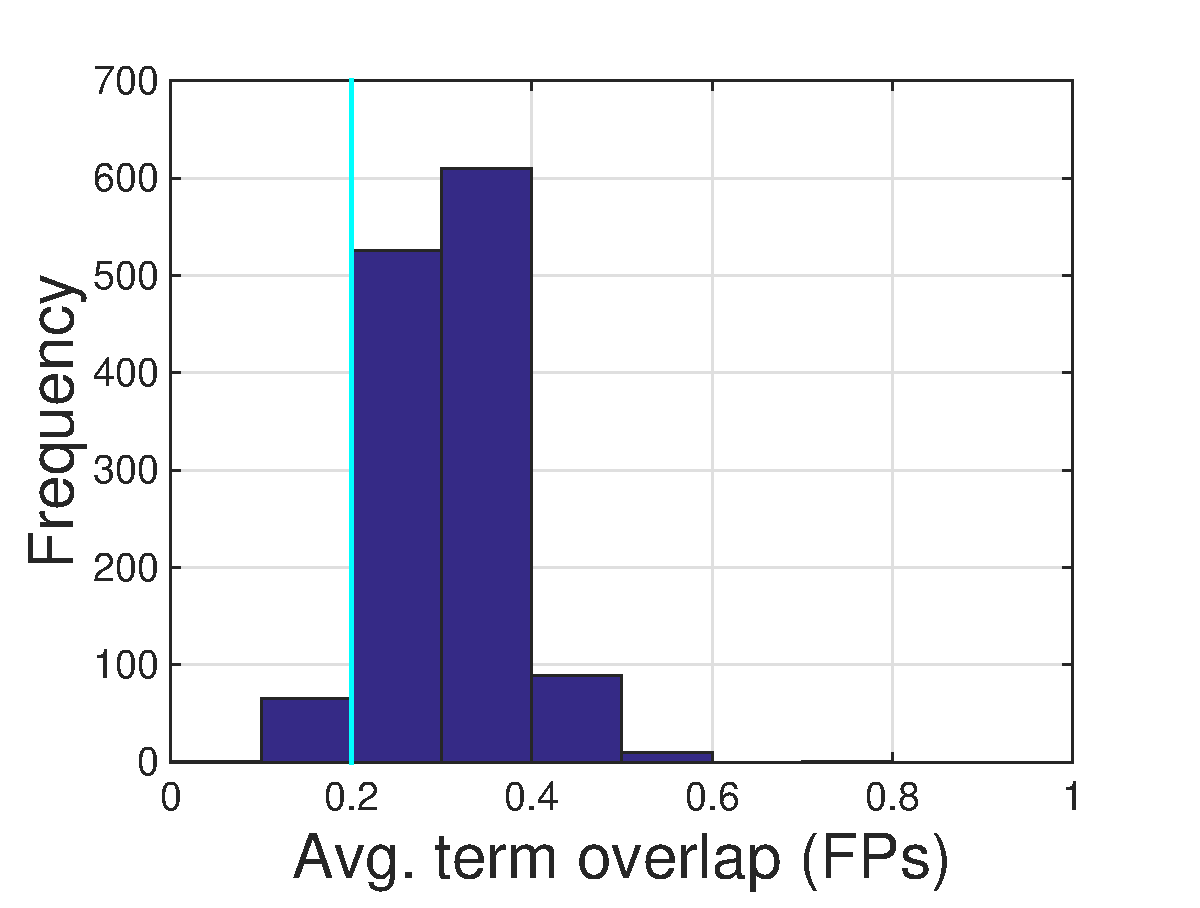
\includegraphics[width=5cm]{figs/to-fps.eps}}\subfigure[{Query and FN patents.}]{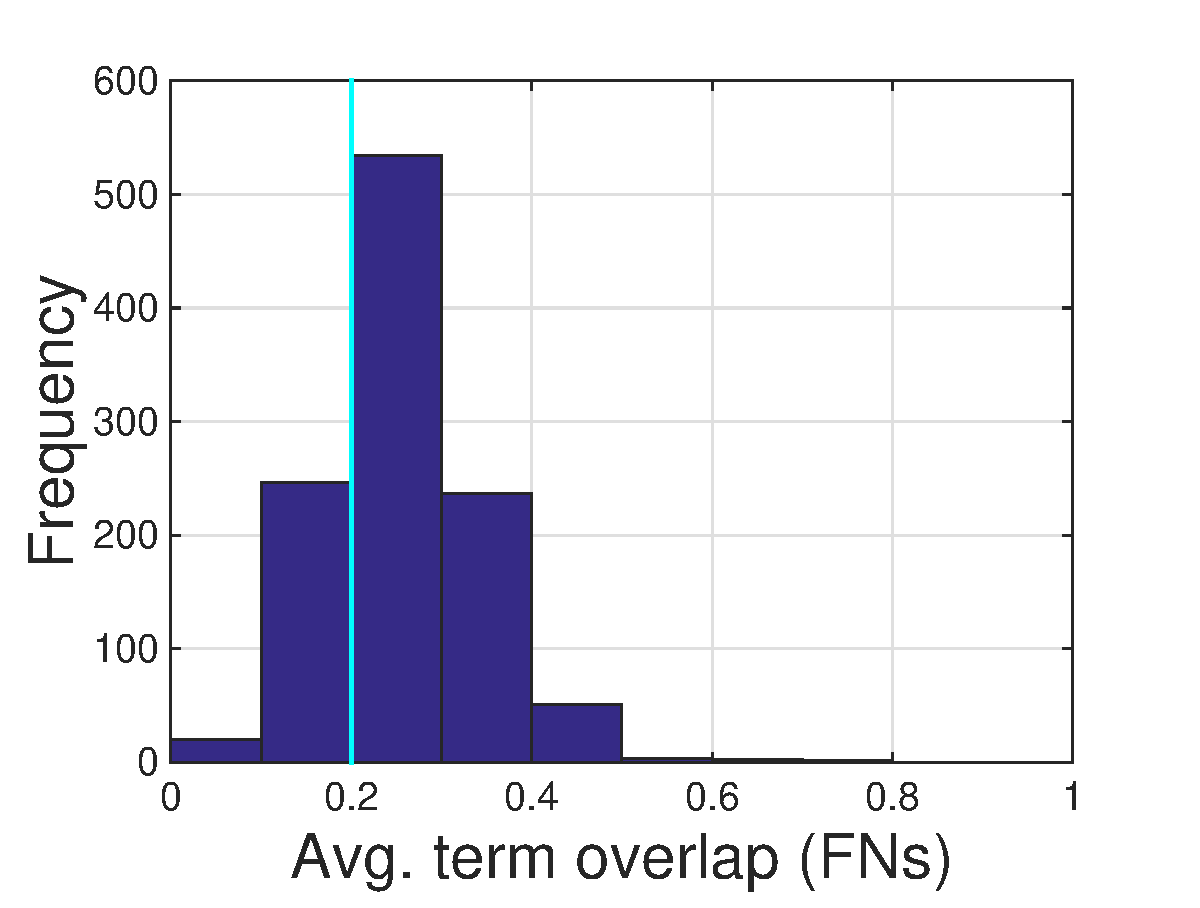
\includegraphics[width=5cm]{figs/to-fns.eps}}
\par\end{centering}

\protect\caption{The distribution of term overlap between the query and documents over 1,303 test queries.}
\label{fig:overlap}
\end{figure}
%%%%%%%%%%%%%%%%%%%%%%%%%%%%%%%%%%%%%%%%%%%%%%%%%%%%%%%%%%%%%%
In summary, this experiment shows that low or zero term match is not the main cause of low effectiveness for patent prior art search.
%%%%%%%%%%%%%%%%%%%%%%%%%%%%%%%%%%%%%%%%%%%%%%%%%%%%%%%%%%%%%%
%%%%%%%%%%%%%%%%%%%%%%%%% SECTION 2 %%%%%%%%%%%%%%%%%%%%%%%%%%
%%%%%%%%%%%%%%%%%%%%%%%%%%%%%%%%%%%%%%%%%%%%%%%%%%%%%%%%%%%%%%
\section{Oracular Relevance Feedback System}
\label{sec:oraculrquery}
A query is optimal if it ranks all relevant documents before
those that are not relevant, that is, it would lead to a ranking with an average precision of 1.0. A query
is most likely to achieve a ranking that is as close to optimal as possible if it contains all terms that
appear in all relevant documents, but explicitly discounts all terms that occur in non-relevant documents~\citep{manning2008introduction}.
Inspired by this fact, we develop an oracular relevance feedback system, which
extracts terms from the judged relevant documents to derive an upper bound on performance of
standard Okapi BM25 and Language Models (LM) retrieval
algorithms for patent prior art search.
%\subsection{Oracular Term Selection}
\subsection{Selecting Useful Terms}
\label{OracularTermSelection}
We aim at identifying the terms, which are considered useful in the query to achieve a ranking that is as close to optimal as possible. For this purpose, 
after an initial run of reference Patent Query, we
calculate an Oracular Relevance Feedback ($\mathit{RF}$) score for each term in the top-100
retrieved documents as follows:
%%%%%%%%%%%%%%%%%%%%%%%%%%%%%%%%%%%%%%%%%%%%%%%%%%%%%%%%%%%%%%
\begin{equation}
RF(t,Q)=Rel(t)-Irr(t) 
 \label{eq:score}
\end{equation}
\begin{displaymath}t\in \lbrace \mbox{terms in top-100 retrieved documents}\rbrace\end{displaymath}
%%%%%%%%%%%%%%%%%%%%%%%%%%%%%%%%%%%%%%%%%%%%%%%%%%%%%%%%%%%%%%
where $ \mathit{Rel(t)} $ is the average term frequency in retrieved relevant patents and $ \mathit{Irr(t)} $ is the average term frequency in retrieved irrelevant patents. We assume words with a positive score are Useful Terms since they are more frequent in relevant patents, while words with a negative score are Noisy Terms as they appear more frequently in irrelevant patents. 

We yield the Oracular Relevance Feedback score to: (i) find a pattern for the system performance versus Useful Terms; (ii) show the term overlap with Useful Terms and Noisy Terms for TP, FN patents; (iii)  examine the existence of Useful Terms in different sections of Patent Query.
%%%%%%%%%%%%%%%%%%%%%%%%%%%%%%%%%%%%%%%%%%%%%%%%%%%%%%%%%%%%%%
\begin{figure}[t!]
\begin{centering}
\subfigure[Useful Terms: $ \{t|RF(t, Q)>0\} $]{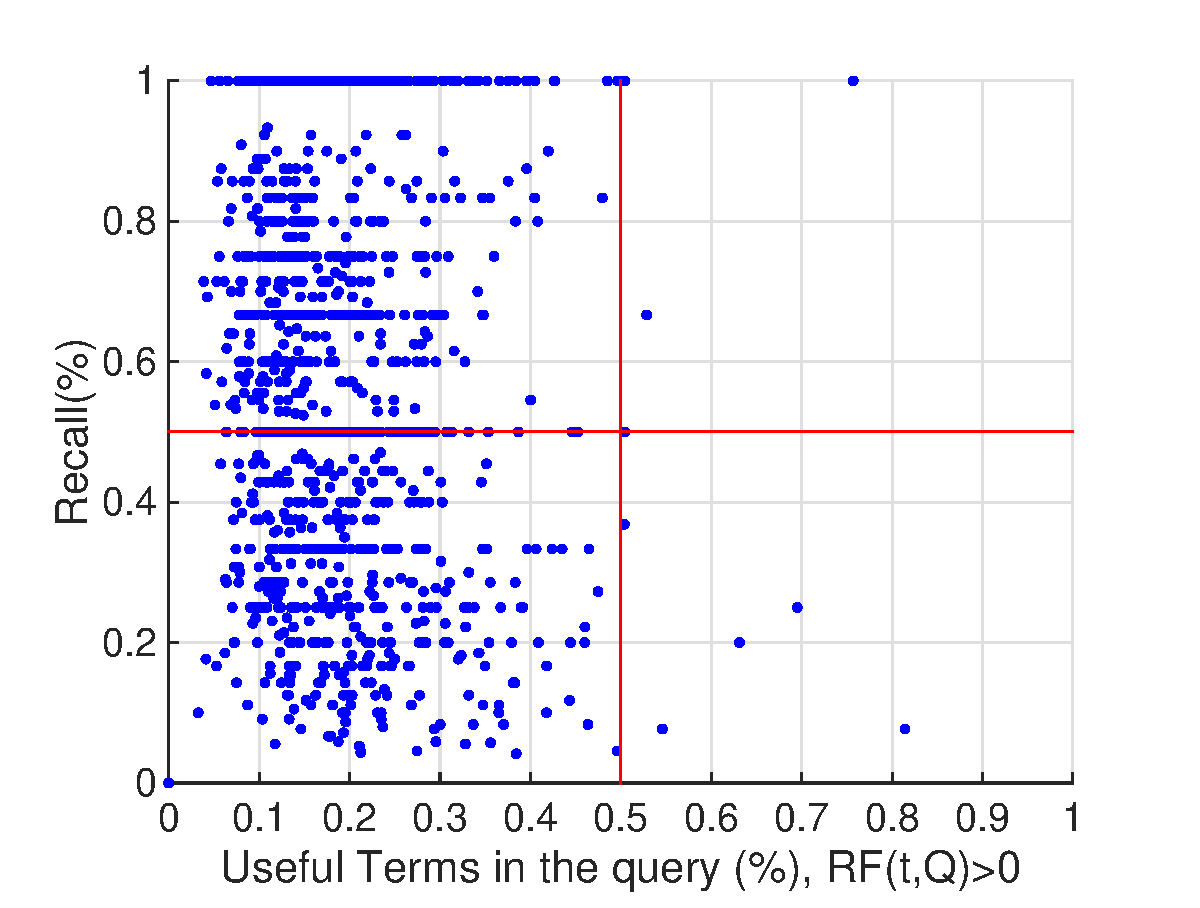
\includegraphics[width=5cm]{figs/greaterthan0-r.eps}} \hspace*{1.5cm} \subfigure[Useful Terms: $ \{t|RF(t, Q)>RF(t_{+median})\} $]{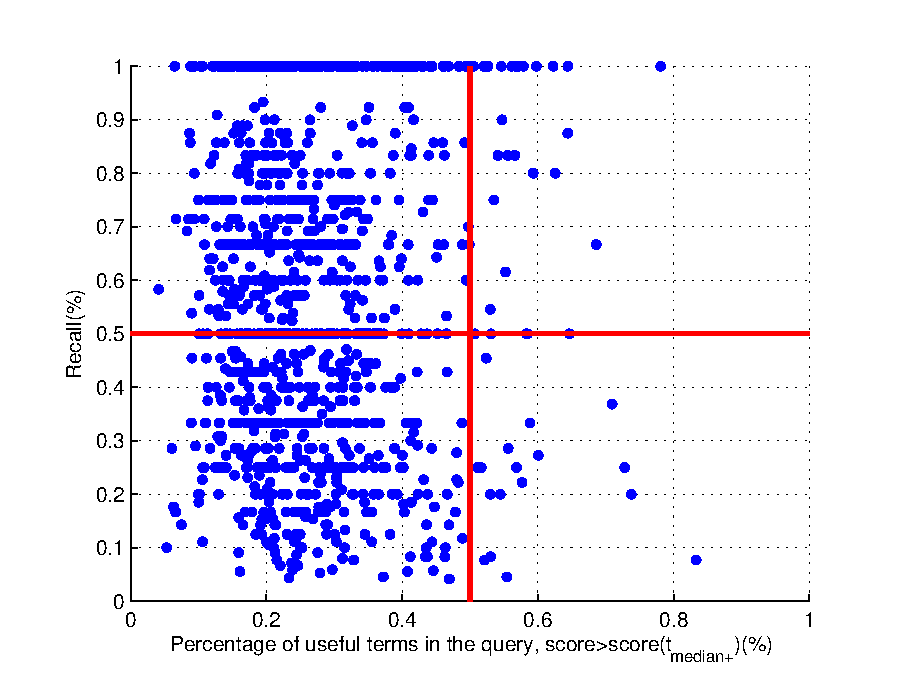
\includegraphics[width=5cm]{figs/greaterthanmedian-r.eps}}\\ \subfigure[{Useful Terms: $ \{t|RF(t, Q)>1 \}$}]{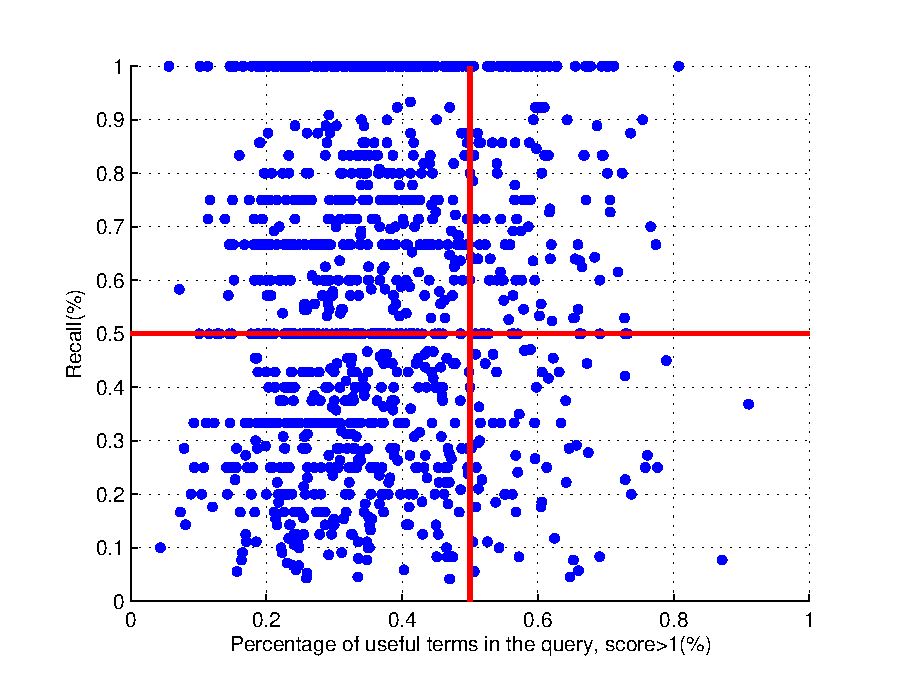
\includegraphics[width=5cm]{figs/greaterthan1-r.eps}} \hspace*{1.5cm} \subfigure[{Useful Terms: top 100 high-scored terms}]{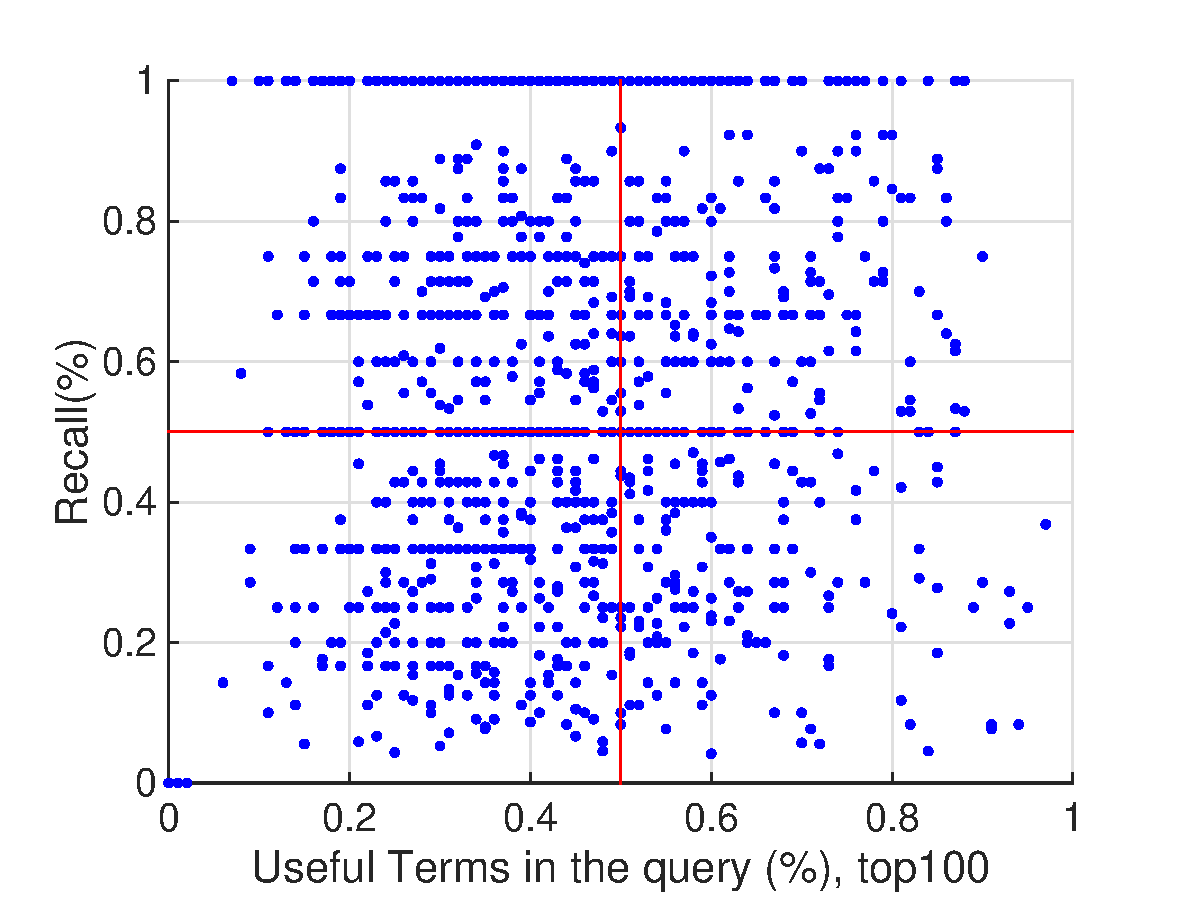
\includegraphics[width=5cm]{figs/top100-r.eps}}\\ \subfigure[{Useful Terms: $ \{t|RF(t,Q)>5 \}$}]{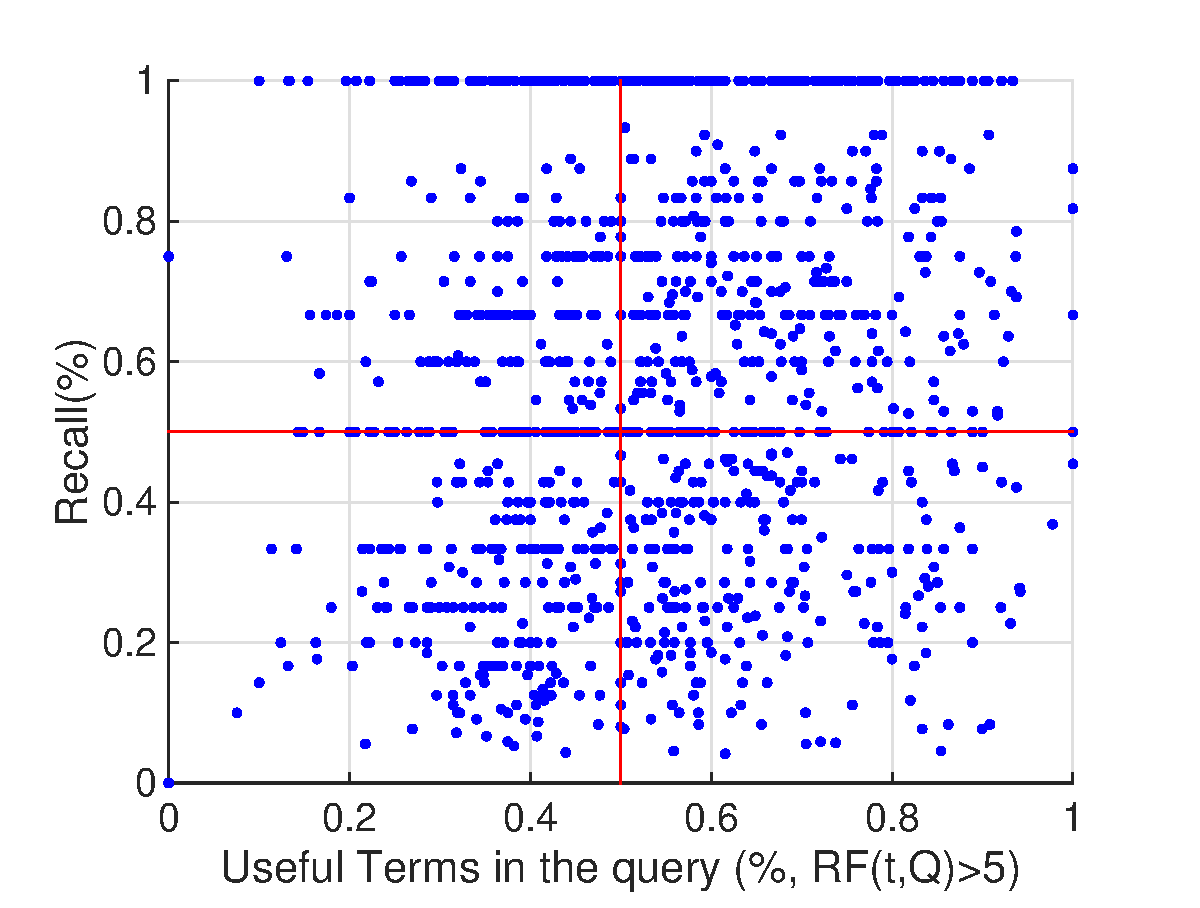
\includegraphics[width=5cm]{figs/greaterthan5-r.eps}} \hspace*{1.5cm} \subfigure[{Useful Terms: $ \{t|RF(t, Q)>10\} $}]{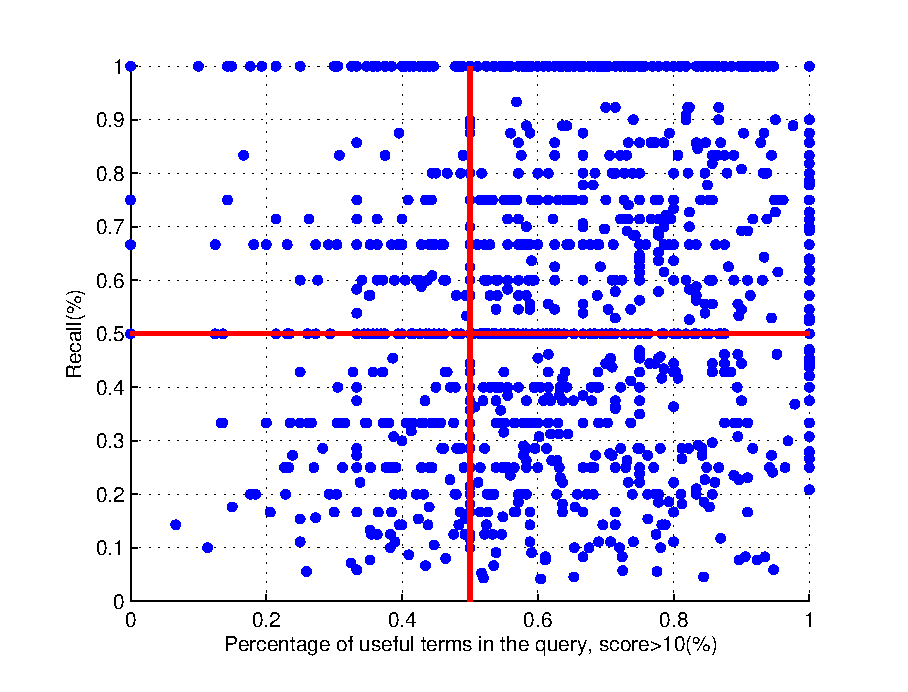
\includegraphics[width=5cm]{figs/greaterthan10-r.eps}}
\par\end{centering}

\protect\caption{Scatter plot of Recall versus the existence of Useful Terms in query.}
\label{fig:overlap-r}
\end{figure}
%%%%%%%%%%%%%%%%%%%%%%%%%%%%%%%%%%%%%%%%%%%%%%%%%%%%%%%%%%%%%%
%%%%%%%%%%%%%%%%%%%%%%%%%%%%%%%%%%%%%%%%%%%%%%%%%%%%%%%%%%%%%%
\begin{figure}[t!]
\begin{centering}
\subfigure[Useful terms: $ \{t|RF(t, Q)>0\} $]{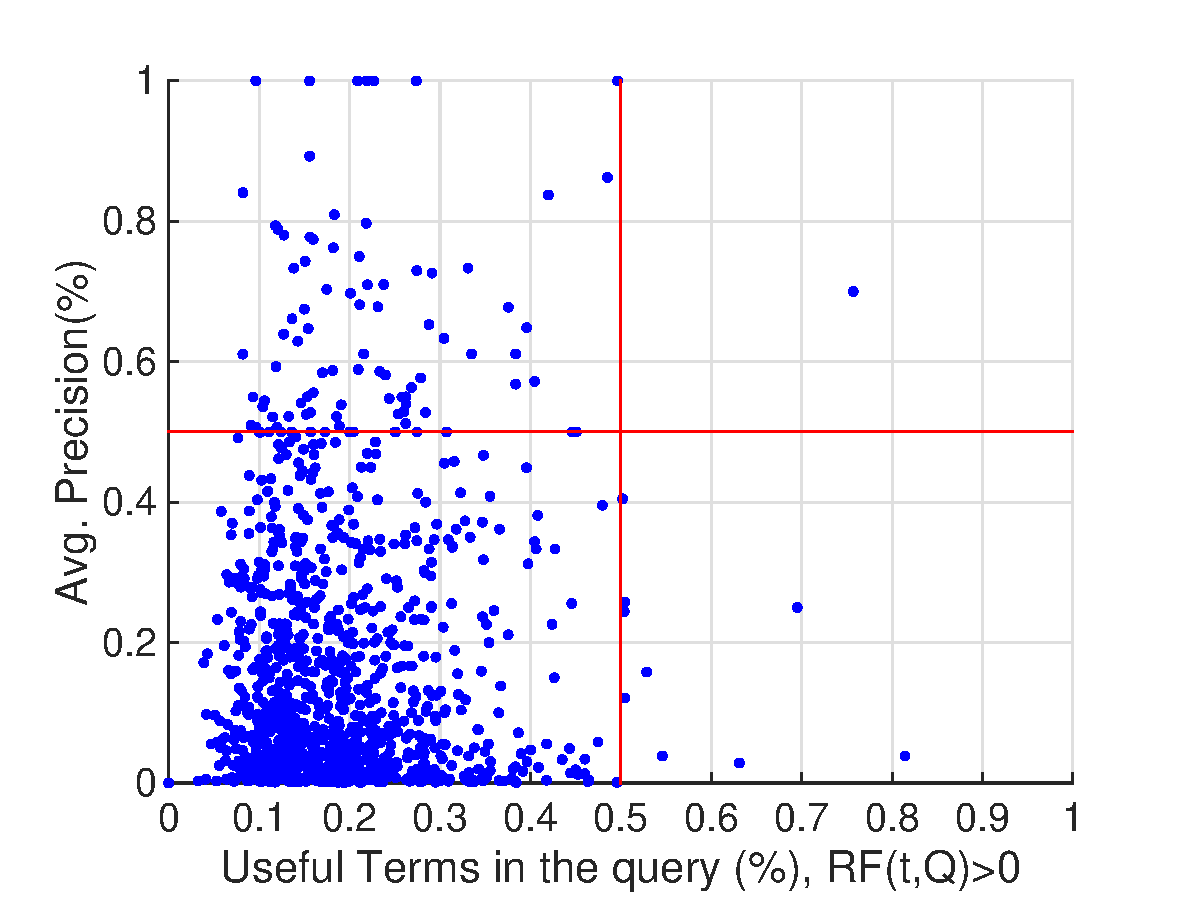
\includegraphics[width=5cm]{figs/greaterthan0-p}} \hspace*{1.5cm} \subfigure[Useful terms: $ \{t|RF(t, Q)>RF(t_{+median}, Q)\} $]{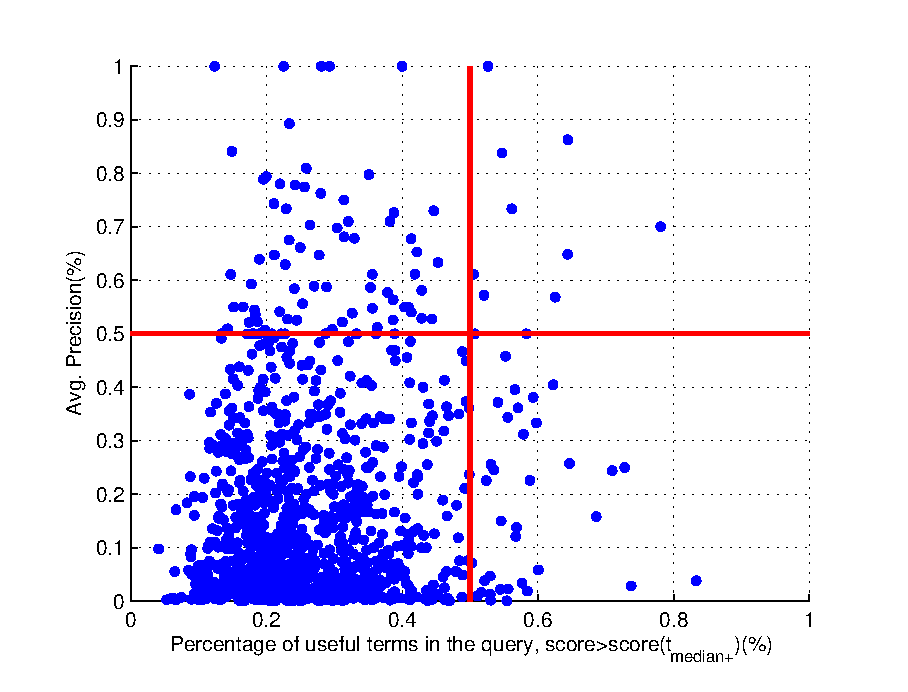
\includegraphics[width=5cm]{figs/greaterthammedian-p.eps}} \\%[-2ex]% 
\subfigure[{Useful terms: $ \{t|RF(t, Q)>1 \}$}]{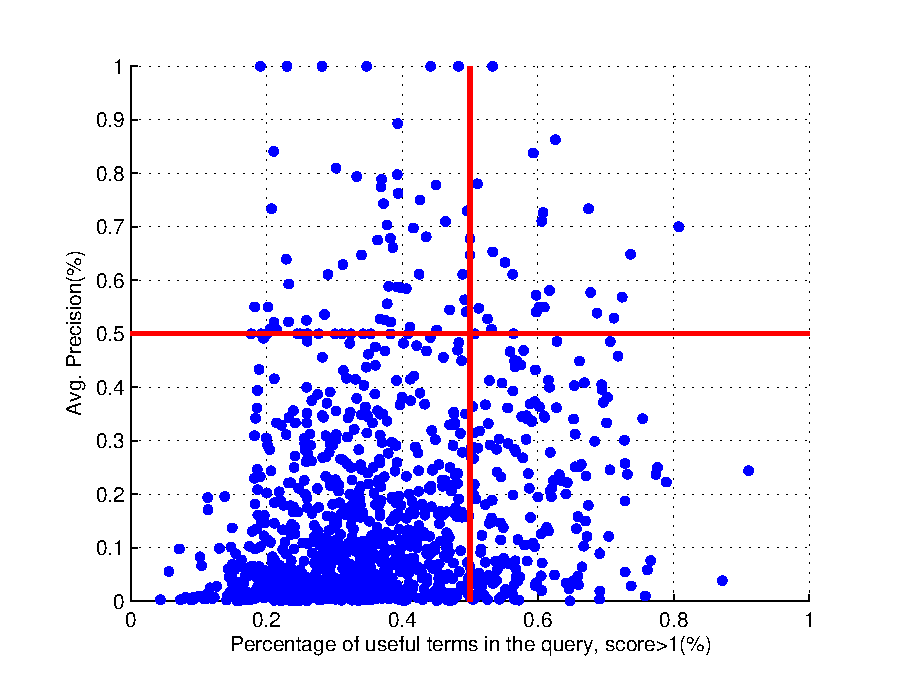
\includegraphics[width=5cm]{figs/greaterthan1-p.eps}} \hspace*{1.5cm} \subfigure[{Useful terms: top 100 high-scored terms}]{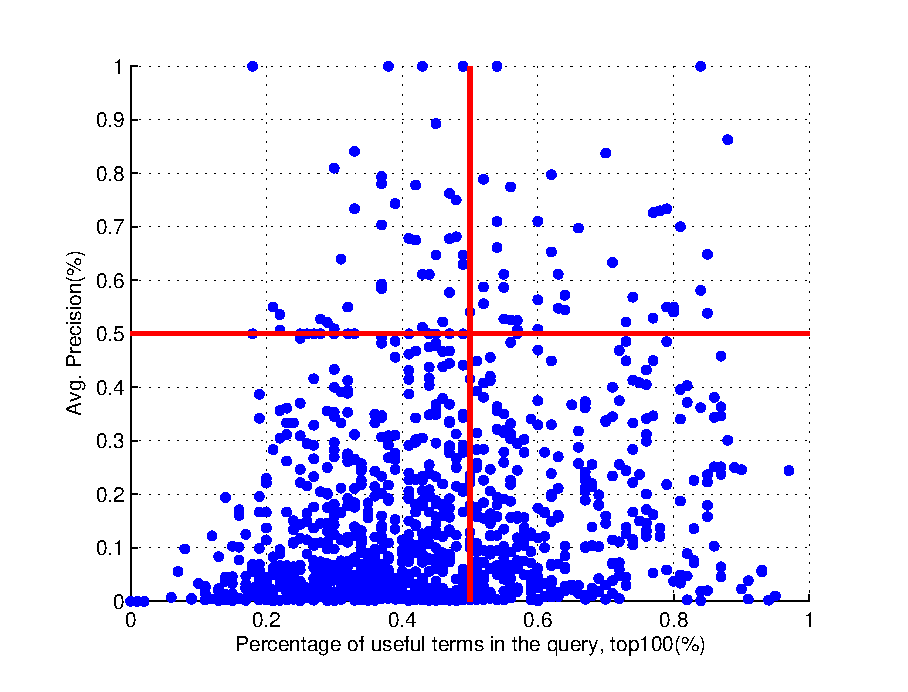
\includegraphics[width=5cm]{figs/top100-p.eps}}\\ %[-2ex]%
\subfigure[{Useful terms: $ \{t|RF(t,Q)>5 \}$}]{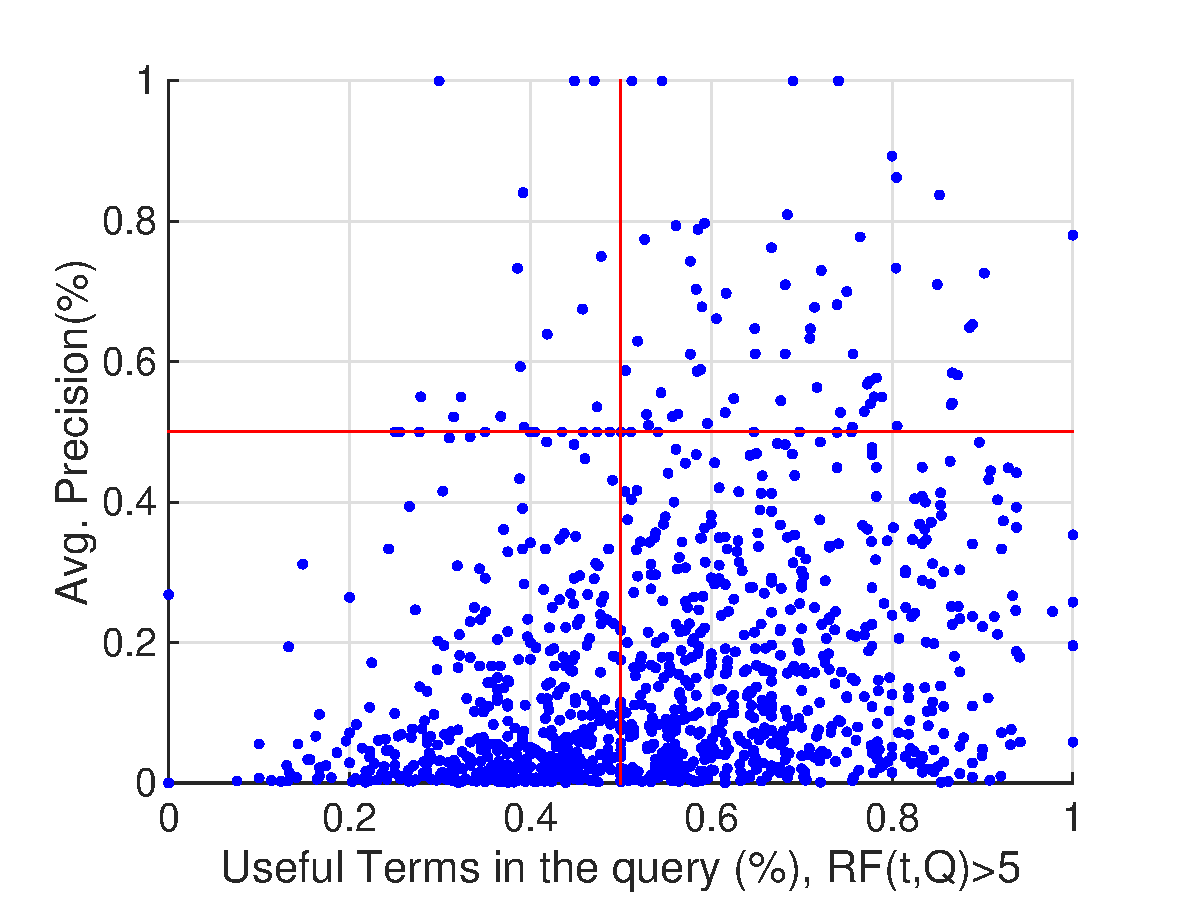
\includegraphics[width=5cm]{figs/greaterthan5-p.eps}} \hspace*{1.5cm} \subfigure[{Useful terms: $ \{t|RF(t, Q)>10\} $}]{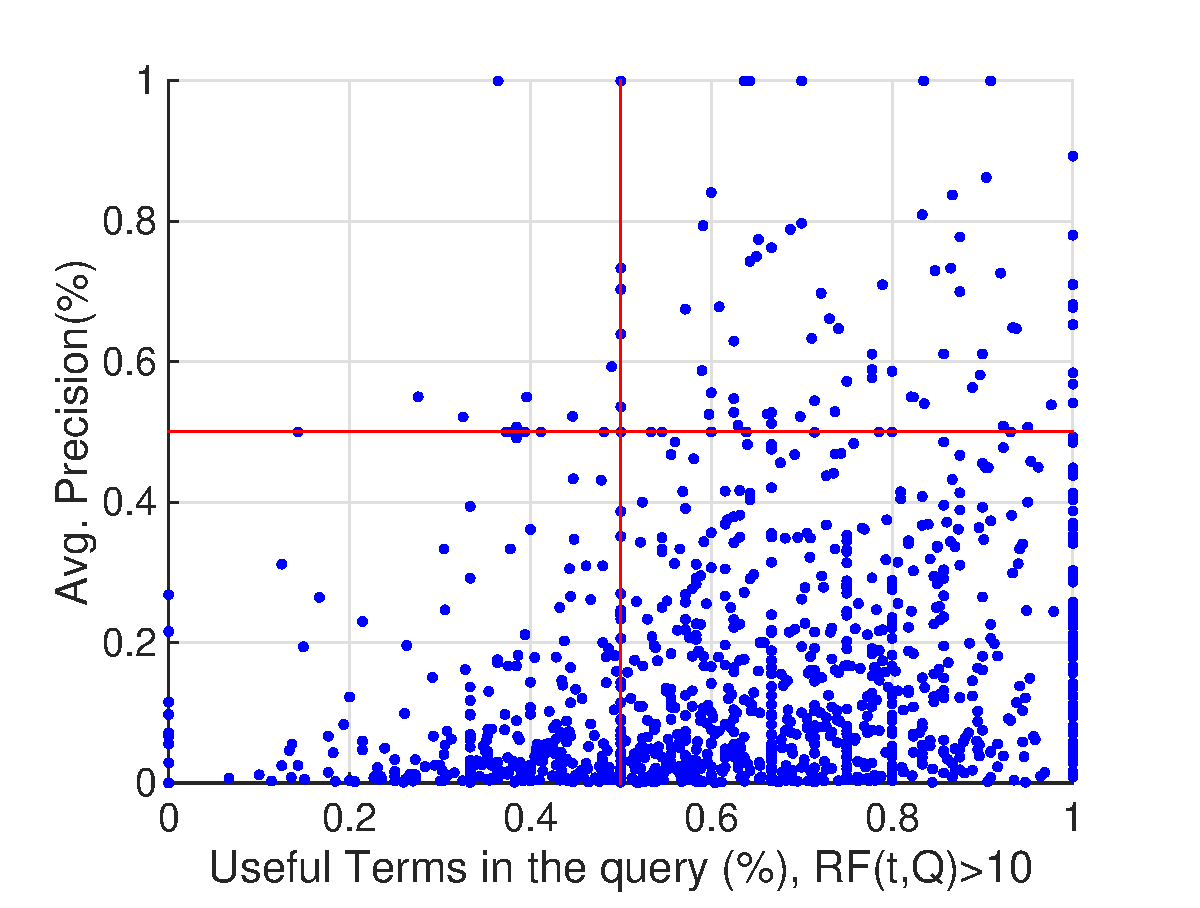
\includegraphics[width=5cm]{figs/greaterthan10-p.eps}}
\par\end{centering}

\protect\caption{Scatter plot of Average Precision versus the existence of Useful Terms in query.}
\label{fig:overlap-p}
\end{figure}
%%%%%%%%%%%%%%%%%%%%%%%%%%%%%%%%%%%%%%%%%%%%%%%%%%%%%%%%%%%%%%
\subsubsection{Performance versus Useful Terms}
\label{PerformanceUsefulTerms}
%\paragraph{Performance versus Useful Terms}
%\ \\
In our first experiment, we investigate whether the existence of more Useful Terms in the reference Patent Query means achieving a higher performance. In other words, we seek for a pattern between the performance and the existence of Useful Terms in initial Patent Query. We define four different criteria to select Useful Terms:
\begin{enumerate}
\item Terms with positive RF scores ($ RF(t, Q)>0) $).
\item Terms with the score higher than the positive median score ($ RF(t, Q)>RF(t_{+median}, Q) $).
\item Terms with the score higher than a constant: 1, 5, and 10 ($ RF(t, Q)>1, 5, 10) $).
\item Top-100 high-scored terms.
\end{enumerate}

Figures~\ref{fig:overlap-r} and~\ref{fig:overlap-p} show the scatter plot of the performance (Average Precision, and Recall) versus the existence of Useful Terms in query. 
We expected to see a higher performance for the queries which contain more Useful Terms and a lower performance for the ones with less Useful Terms. However, unlike our first assumption, we do not see any correlation between the performance and the presence of Useful Terms in the query. The pattern for the recall is irregular while there is a very weak correlation between Average Precision and Useful Terms for top-scored words ($RF(t, Q)>10$). This experiment explicitly indicates that term mismatch is not the main reason for low effectiveness of prior art search. 
\subsubsection{Term Overlap with Useful Terms and Noisy Terms}
%\paragraph{Term Overlap with Useful Terms and Noisy Terms}
%\ \\
In the second experiment, we check the term overlap with Useful Terms and Noisy Terms for TP and FP patents. Figure \ref{fig:usefulnoisy} shows that relevant patents have a higher term overlap with the Useful Terms while irrelevant patents have a higher term overlap with the Noisy Terms. This experiment shows that Noisy Terms are the main reason that irrelevant patents are retrieved at top of the list. 
%%%%%%%%%%%%%%%%%%%%%%%%%%%%%%%%%%%%%%%%%%%%%%%%%%%%%%%%%%%%%%
\begin{figure}[t!]
\begin{centering}
\subfigure[TPs]{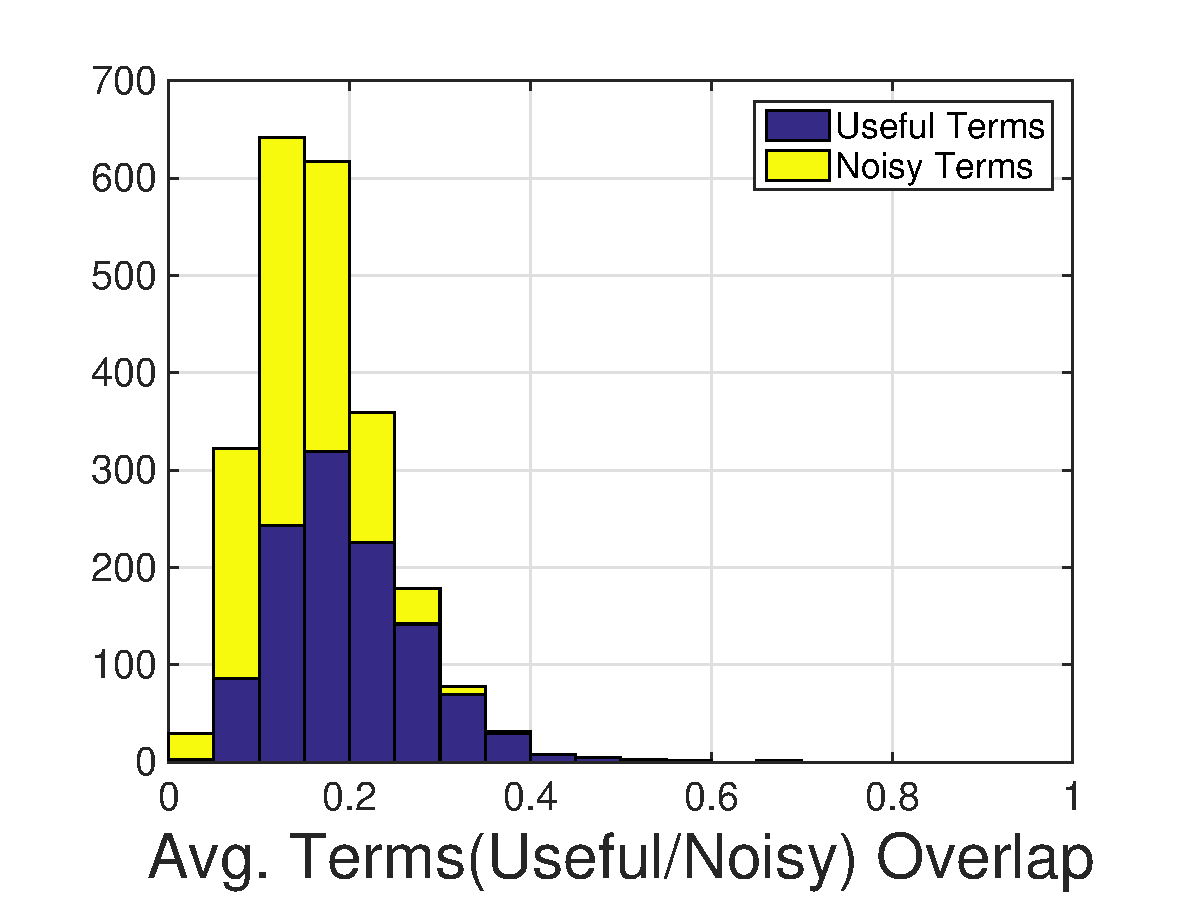
\includegraphics[width=6cm]{figs/stackedTPs.eps}} \hspace*{1.5cm} \subfigure[FPs]{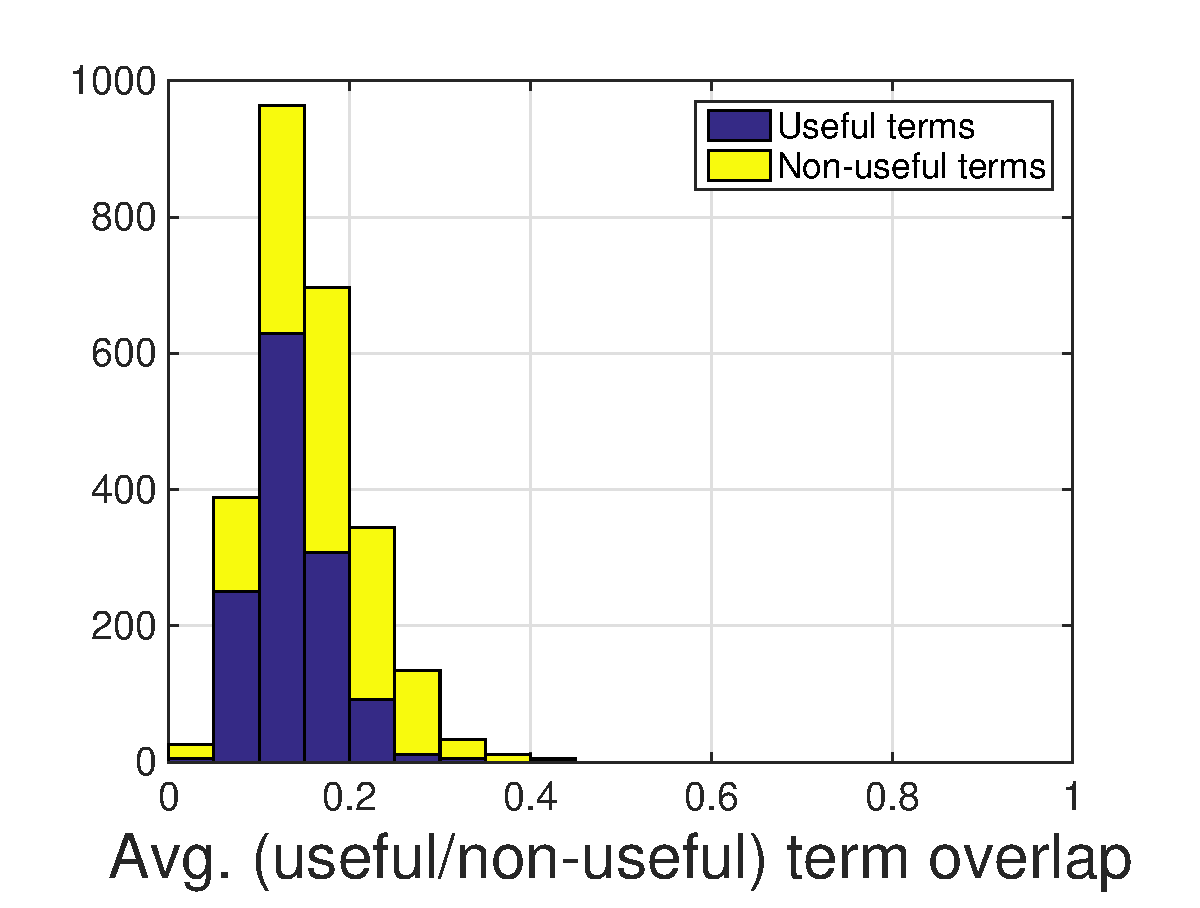
\includegraphics[width=6cm]{figs/stackedFPs.eps}} 
\par\end{centering} 

\protect\caption{The distribution of the term overlap between the query and Useful Terms/Noisy Terms in TPs and FPs. Relevant patents have higher term overlap with Useful Terms while irrelevant patents have higher term overlap with Noisy Terms.}
\label{fig:usefulnoisy}
\end{figure}
%%%%%%%%%%%%%%%%%%%%%%%%%%%%%%%%%%%%%%%%%%%%%%%%%%%%%%%%%%%%%%
%We hypothesized that a query, formulated by only the \textit{ useful terms}, is the best possible query we can make since they are all frequent in relevant patents but rare in irrelevant ones. 
\subsubsection{Useful Terms in Different Sections of Patents}
%\paragraph{Useful Terms in Different Sections of Patents}
%\ \\
Patents are structured documents containing Title, Abstract, Description, and Claims (section~\ref{StructureofPatents}). In this experiment, we investigate Useful Terms in different sections of patents. 
Table (\ref{tab:usefultermsinsections}) shows the average number of Useful Terms in different sections of Patent Query.  
As it can be seen, Description has the highest number of useful terms in both cases where RF score threshold ($ \tau $) is `0' and `1'. When $ \tau = 0 $, the average number of the Useful Terms in Description is quite twice of when $ \tau = 1 $. Compared to other sections, Description contains more Useful Terms, which proves why we achieved higher performance querying with Description (Section~\ref{sec:settings}).
Table (\ref{tab:usefultermsinsections-p}) shows the average percentage of Useful Terms in different sections of Patent Query. It shows that, overall, Useful Terms constitute less than 50\% of the whole words in each section of Patent Queries. For example, we can see that only 27\% of the whole Patent Query in average are Useful Terms and the rest are irrelevant terms. 

%\subsubsection{Useful Terms in Different Sections}
%%%%%%%%%%%%%%%%%%%%%%%%%%%%%%%%%%%%%%%%%%%%%%%%%%%%%%%%%%%%%%
\begin{table*}[t!]
  \begin{center}
   \caption{Average number of Useful Terms in the different sections of Patent Query}
  \input table/usefultermsinsections.tex   
  \label{tab:usefultermsinsections}
  \end{center}  
\end{table*}
%\FloatBarrier
%%%%%%%%%%%%%%%%%%%%%%%%%%%%%%%%%%%%%%%%%%%%%%%%%%%%%%%%%%%%%%
%%%%%%%%%%%%%%%%%%%%%%%%%%%%%%%%%%%%%%%%%%%%%%%%%%%%%%%%%%%%%%
\begin{table*}[t!]
  \begin{center}
   \caption{Average percentage of Useful Terms in the different sections of Patent Query}
  \input table/usefultermsinsections-p.tex   
  \label{tab:usefultermsinsections-p}
  \end{center}  
\end{table*}
%%%%%%%%%%%%%%%%%%%%%%%%%%%%%%%%%%%%%%%%%%%%%%%%%%%%%%%%%%%%%%

\subsection{Oracular Query Formulation}
\label{sec:OracularQueryFormulation}
As it explained in section~\ref{PerformanceUsefulTerms}, we could not find a pattern for the performance and the existence of the Useful Terms in Patent Query.
In this section, we examine the system effectiveness for queries formulated by terms selected by Oracular Relevance Feedback ($\mathit{RF}$) system.
We formulate two different Oracular Queries.

The first query is formulated by selecting terms in the top-100 retrieved documents using Oracular Relevance Feedback score and we call it Oracular Query:
%%%%%%%%%%%%%%%%%%%%%%%%%%%%%%%%%%%%%%%%%%%%%%%%%%%%%%%%%%%%%%
\begin{equation}
Oracular \; Query = \{t \in top-100|RF(t, Q)>\tau\}   
 \label{eq:score}
\end{equation}
%%%%%%%%%%%%%%%%%%%%%%%%%%%%%%%%%%%%%%%%%%%%%%%%%%%%%%%%%%%%%% 
We empirically seek to evaluate the threshold $\tau$ on $RF(t,Q)$ and query size yielding the best oracular query.
Table~\ref{tab:optquery} and Figure~\ref{fig:oracular-a} show that the Oracular Query far outperform the baseline query (reference Patent Query), and it approximately performs twice as well on the PATATRAS system, the best competitor in CLEF-IP 2010 system. In Table~\ref{tab:optquery}, we also compare the influence of weighed and unweighed terms for both baseline query and Oracular Query. It can be seen that weighing terms in Patent Query with their frequency helps the performance while weighing terms in Oracular Query with $RF(t, Q)$ harms the performance. 
Figure \ref{fig:oracular-a} shows how the performance changes by the values of $\tau$. We remark two important facts: 
\begin{enumerate}
\item Including slightly Noisy Terms (i.e., $\tau$ just slightly less than 0) leads in an unexpected steep drop-off in performance.  
\item We achieve the highest MAP for the Oracular Query formulated by selecting the terms with $RF(t, Q)>0$.
\end{enumerate}
Figure~\ref{fig:oracular-b} shows that the performance increases notably when we include terms up to 200 while formulating a query, but it remains quit unchanged when we include more than 200 terms. 
%%%%%%%%%%%%%%%%%%%%%%%%%%%%%%%%%%%%%%%%%%%%%%%%%%%%%%%%%%%%%%
\begin{table}[t!]
  \begin{center}
  \scriptsize
   \caption{Performance for the Patent Query, Oracular Query, and Top CLEF-IP 2010 (PATATRAS).}
   \vspace*{1ex}
  \input table/optquery.tex   
  \label{tab:optquery}
  \end{center}  
\end{table}
%%%%%%%%%%%%%%%%%%%%%%%%%%%%%%%%%%%%%%%%%%%%%%%%%%%%%%%%%%%%%%
%%%%%%%%%%%%%%%%%%%%%%%%%%%%%%%%%%%%%%%%%%%%%%%%%%%%%%%%%%%%%%
\begin{figure}[t!]
\begin{centering}
\subfigure[Oracular Query performance versus the threshold $\tau$.\label{fig:oracular-a}]{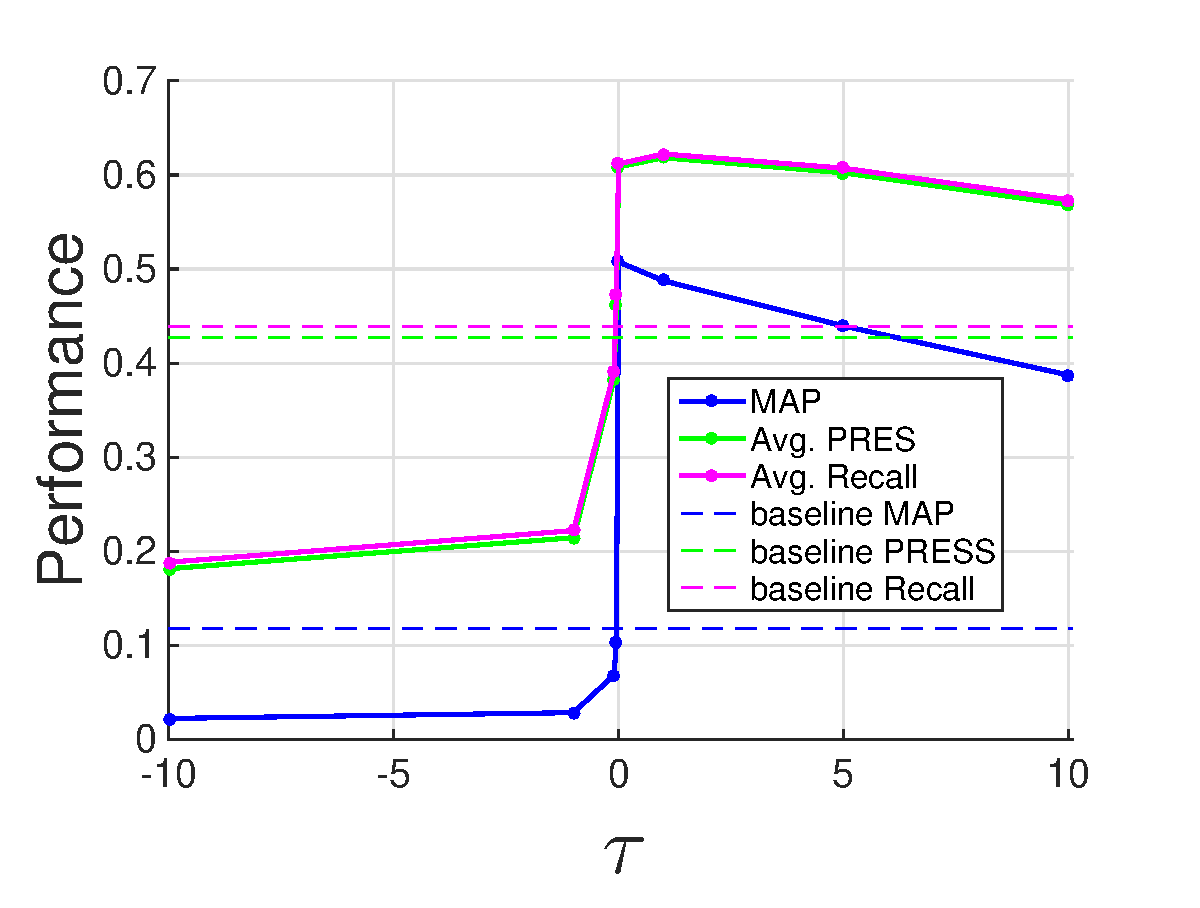
\includegraphics[width=6cm]{figs/oracularq.eps}} \hspace*{1.5cm} \subfigure[Oracular Query performance versus the query size.\label{fig:oracular-b}]{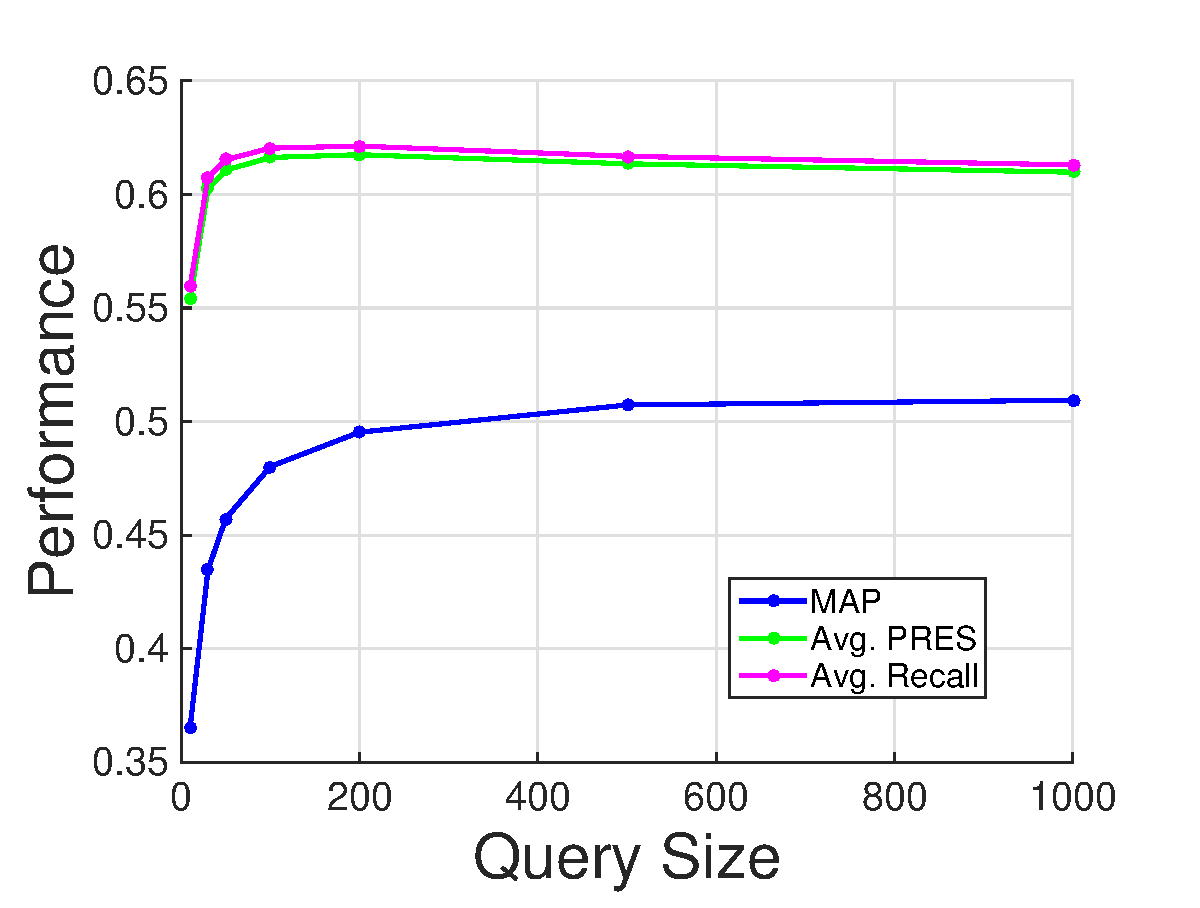
\includegraphics[width=6cm]{figs/oracularq-size.eps}} 
\par\end{centering} 
\protect\caption{Oracular Query performance versus various values of the threshold $\tau$ and query size}
\label{fig:oracular}
\end{figure}
%%%%%%%%%%%%%%%%%%%%%%%%%%%%%%%%%%%%%%%%%%%%%%%%%%%%%%%%%%%%%%

%Next, inspired by Maxwell and Croft's work~\citep{maxwell2013compact} that emphasise on the importance of query words, 
We seek to establish that the terms within a reference Patent Query are sufficient for a strong performance, so, we formulate the second query by selecting oracular terms that also occur in the reference patent query We call it Oracular Patent Query:
%%%%%%%%%%%%%%%%%%%%%%%%%%%%%%%%%%%%%%%%%%%%%%%%%%%%%%%%%%%%%%
\begin{equation}
 Oracular \; Patent \; Query = \{t\in Q|RF(t, Q)>\tau\}   
 \label{eq:score}
\end{equation}
%%%%%%%%%%%%%%%%%%%%%%%%%%%%%%%%%%%%%%%%%%%%%%%%%%%%%%%%%%%%%%
%%%%%%%%%%%%%%%%%%%%%%%%%%%%%%%%%%%%%%%%%%%%%%%%%%%%%%%%%%%%%%
\begin{figure}[t!]
\begin{centering}
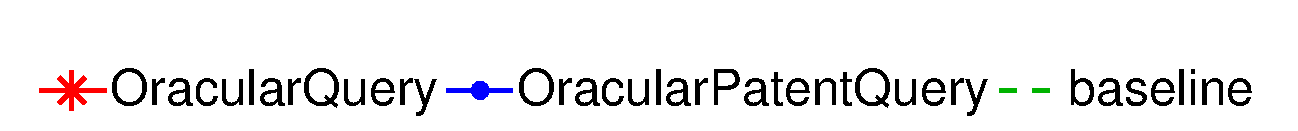
\includegraphics[width=9cm]{figs/l1}
\par\end{centering}

\begin{centering}
\subfigure[Mean Average Precision $\tau$.\label{fig:oracularpq-a}]{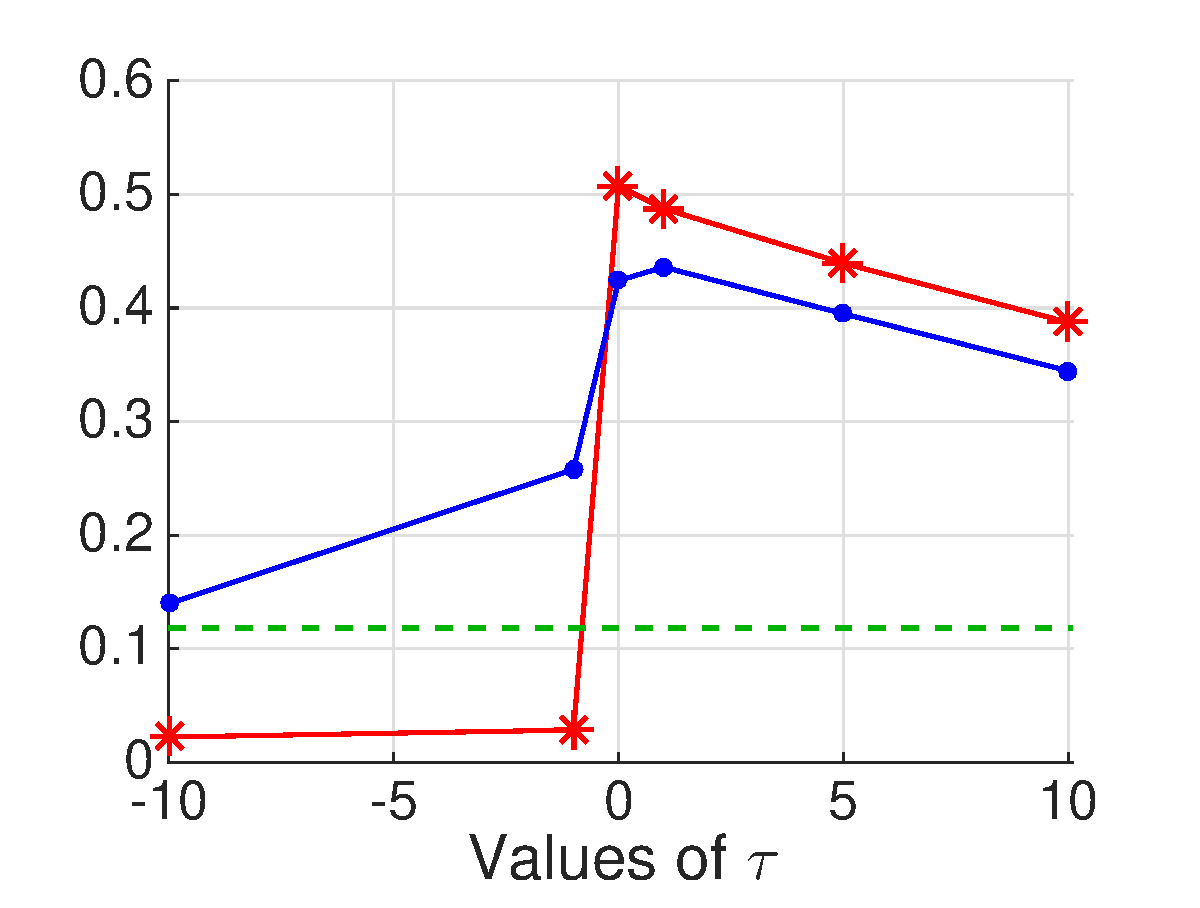
\includegraphics[width=6cm]{figs/fig1_map.eps}} 
\hspace*{1.5cm} \subfigure[Average Recall\label{fig:oracularpq-b}]{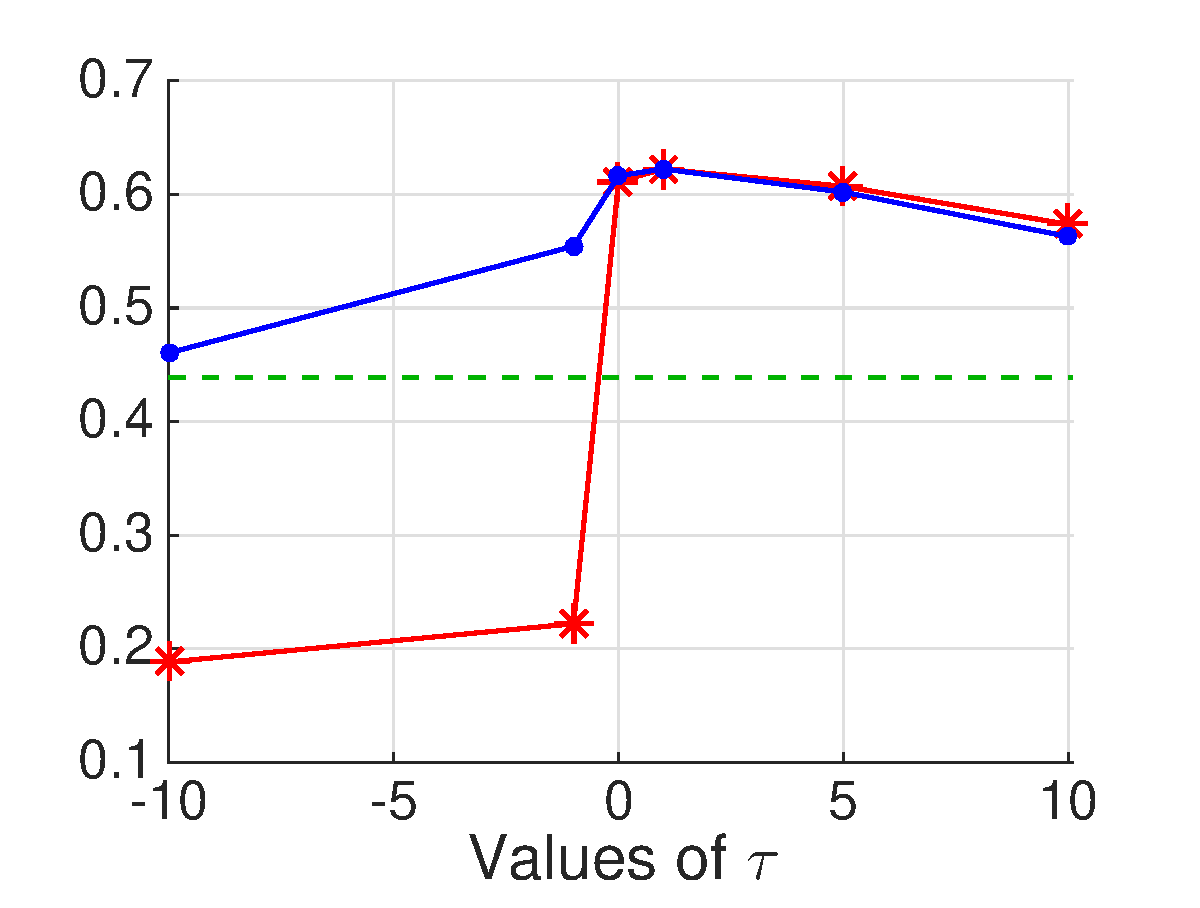
\includegraphics[width=6cm]{figs/fig1_recall.eps}} 
\par\end{centering} 

\protect\caption{Comparing the performance of Oracular Query and Oracular Patent Query for various values of the threshold $\tau$}
\label{fig:oracularpq}
\end{figure}
\begin{figure}[t!]
   \centering
   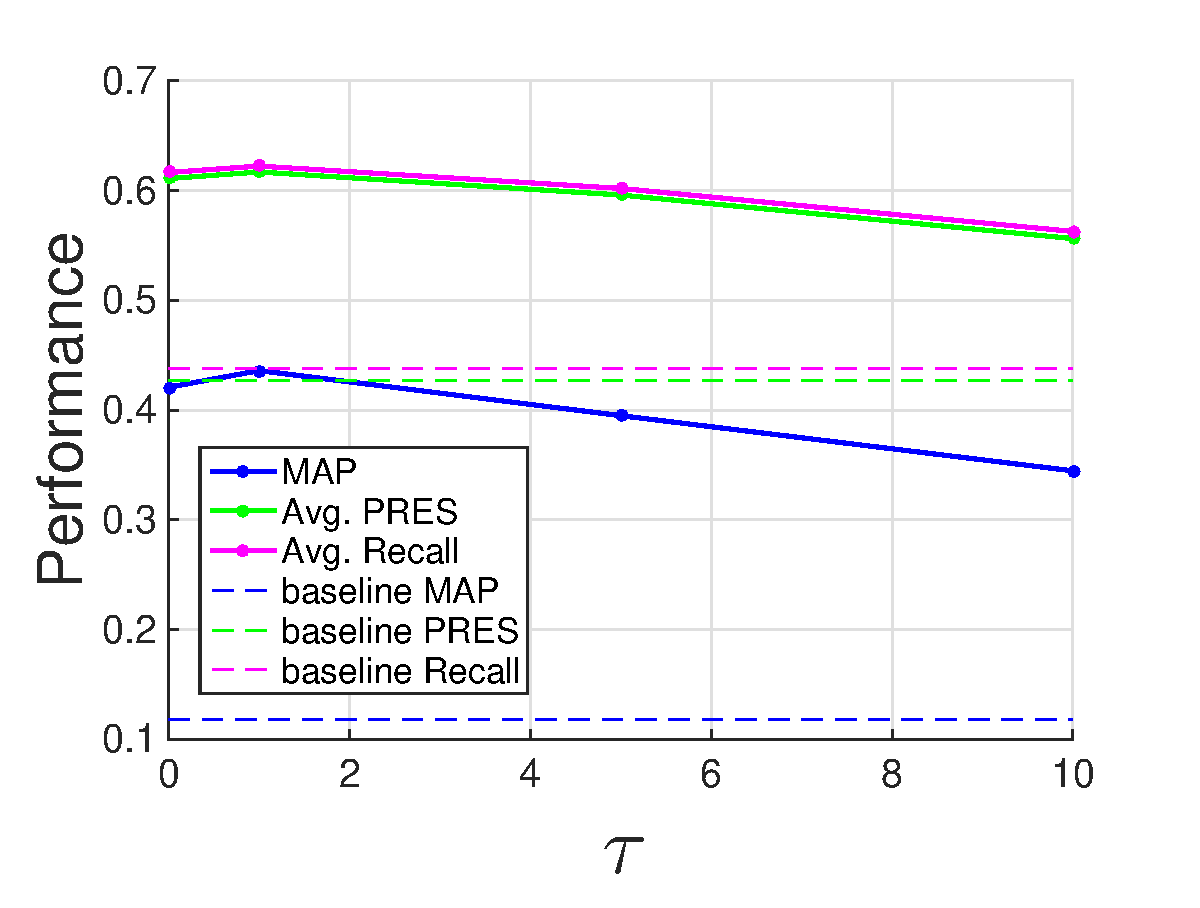
\includegraphics[width=0.50\textwidth,height=55mm]{figs/oracularpq.eps}
   \caption{oracular patent query performance versus the threshold $\tau$.}   
   \label{fig:oracularpq} 
\end{figure}
%%%%%%%%%%%%%%%%%%%%%%%%%%%%%%%%%%%%%%%%%%%%%%%%%%%%%%%%%%%%%%
As it has been shown in Table~\ref{tab:optquery} and Figure~\ref{fig:oracularpq}, the system performance for the Oracular Patent Query is also considerably improved compared to the baseline and PATATRAS.
% though MAP is slightly less than Oracular Query. 
The results indicate that the Patent Query has sufficient terms for an improved performance. 
We compare MAP and Recall for both Oracular Query and Oracular Patent Query in Figure~\ref{fig:oracularpq}. 
On one hand, We notice that MAP for Oracular Patent Query is slightly less than MAP for Oracular Query. We justify that it is due to some extra terms in top-100 vocabulary set that they are absent within the Patent Query. On the other hand, Oracular Patent Query performance drops slower for negative values of $\tau$, which shows that Oracular Patent Query contains less Noisy Terms than Oracular Query. 
This explains why query expansion techniques is not too effective for patent prior art search. We also conclude that the the existence of the Noisy Terms is the main cause of low effectiveness in prior art search.  

To recap, our experiments related to Oracular Relevance Feedback system
suggest two important conclusions: 
\begin{enumerate}
\item Query reduction should suffice for effective prior art patent retrieval; and 
\item Very precise methods for eliminating poor query terms in the reduction process are required.
\end{enumerate}

%\subsection{Discriminative Words}
%\label{sec:discriminative}
%
%\subsection{RF Optimal Query Formulation}
%\label{sec:formulation}

%%%%%%%%%%%%%%%%%%%%%%%%%%%%%%%%%%%%%%%%%%%%%%%%%%%%%%%%%%%%%%
%%%%%%%%%%%%%%%%%%%%%%%%% SECTION 3 %%%%%%%%%%%%%%%%%%%%%%%%%%
%%%%%%%%%%%%%%%%%%%%%%%%%%%%%%%%%%%%%%%%%%%%%%%%%%%%%%%%%%%%%%
\section{Query Reduction: Approximating the Oracular Patent Query}
\label{sec: QR}
The gain achieved using the Oracular Patent Query method motivates us to explore various methods to approximate the terms
selected by this query without ``peeking at the answers'' provided by
the actual relevance judgements.  We first attempt this via fully
automated methods and then proceed to evaluate semi-automated methods
based on interactive relevance feedback methods.
\subsection{Automated Reduction}
\label{AutomatedReduction}
For automated reduction we first examine three simple approaches, then we apply Pseudo Relevance Feedback for query term selection.  
\subsubsection{Simple Query Reduction Approaches}
%%%%%%%%%%%%%%%%%%%%%%%%%%%%%%%%%%%%%%%%%%%%%%%%%%%%%%%%%%%%%%
%\begin{figure}[t!]
%\begin{centering}
%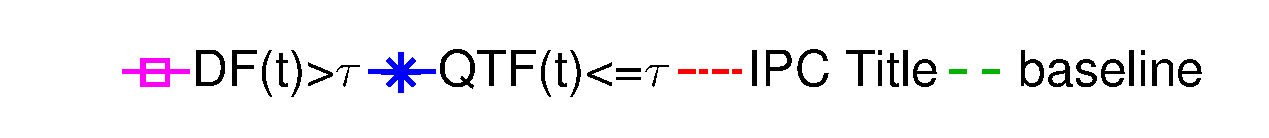
\includegraphics[width=9cm]{figs/l3}
%\par\end{centering}
%
%\begin{centering}
%\subfigure[Mean Average Precision.]{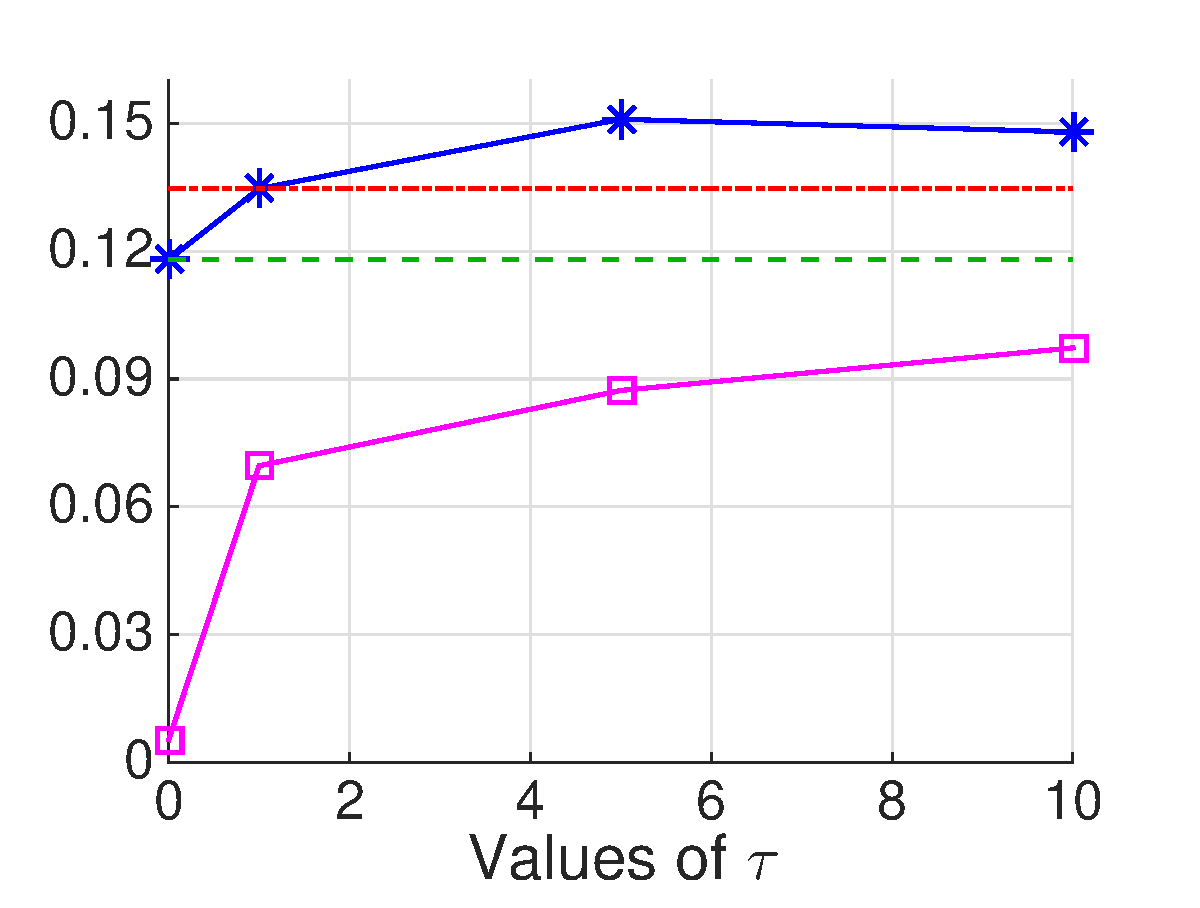
\includegraphics[width=6cm]{figs/fig3_map}} \hspace*{1.5cm} \subfigure[Average Recall.]{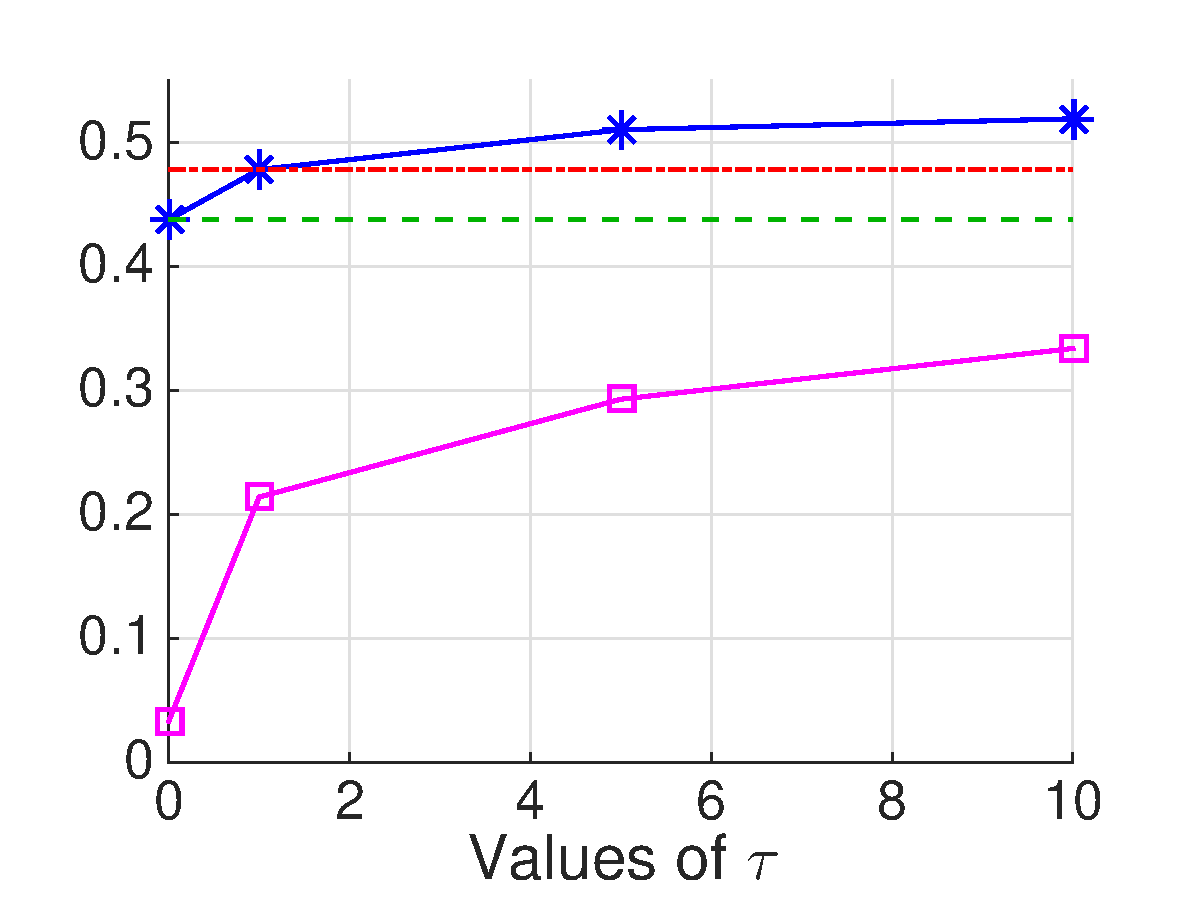
\includegraphics[width=6cm]{figs/fig3_recall}} 
%\par\end{centering} 
%
%\protect\caption{Comparing system performance for three different query reduction approaches and their changes with a threshold $\tau$.}
%\label{fig:combinedapproach}
%\end{figure}
%%%%%%%%%%%%%%%%%%%%%%%%%%%%%%%%%%%%%%%%%%%%%%%%%%%%%%%%%%%%%%
\label{SimpleApproaches}
We, first, apply three simple approaches to reduce the initial patent queries aiming at approximating the Oracular Patent Query: (i) removing document frequent terms; (ii) removing less frequent terms in Patent Query; (iii) Removing Terms in IPC Titles.
\paragraph{Removing Document Frequent Terms}
\ \\
In standard IR, removing terms appearing highly frequently across documents in the collection can improve retrieval effectiveness~\citep{manning2008introduction}. Inspired by this fact, we hypothesize that we will improve the performance by pruning out highly frequent words in top-100 retrieved documents after an initial run of Patent Query. To identify highly frequent terms, we calculate the average term frequency over top-100 documents for each word and we call it Document Frequent (DF) score, as follows:
%%%%%%%%%%%%%%%%%%%%%%%%%%%%%%%%%%%%%%%%%%%%%%%%%%%%%%%%%%%%%%
\begin{equation}
 DF(t, Q)=\frac{1}{100}\sum_{d_i\in  D} TF(t, d_i)    
 \label{eq:df}
\end{equation}
where $D=\{d\in \mbox{Top-100 retrieved documents}\}$, and $TF(t, d_i)$ is the term frequency of each term in document $d_i$.
%\begin{displaymath}   t\in \lbrace \mbox{terms in top-100 retrieved documents}\rbrace\end{displaymath}
%%%%%%%%%%%%%%%%%%%%%%%%%%%%%%%%%%%%%%%%%%%%%%%%%%%%%%%%%%%%%%

We remove words with DF score higher than $\tau$ ($DF(t, Q)>\tau$) from Patent Query. Figure~\ref{fig:combinedapproach} illustrates how the performance change by different values of the threshold $\tau$ illustrates that removing document frequent words for different threshold $\tau$ hurts the performance (magenta line). As it can be seen, the performance converges with the baseline performance when $\tau$ goes higher (e.g., 500). This means that there is no term with such a high DF score, and we do not empirically remove any term from the Patent Query. Overall, removing document frequent terms from Patent Query does not consider an appropriate approach since it ruins the performance. 
\paragraph{Removing Less Frequent Terms in Patent Query}
\ \\
Frequent terms inside long and verbose queries are considered important~\citep{maxwell2013compact}. However, we hypothesise that we may improve the effectiveness by removing terms appearing less frequently in the Patent Query. Therefore, we remove terms with the frequency less than the threshold $\tau$ ($QTF(t)<=\tau$ ). The blue line in Figure~\ref{fig:combinedapproach} indicates that the performance gets slightly better than the baseline when we remove less frequent terms in Patent Query. As it can be seen the best MAP achieved when $\tau=5$. 
%In this approach the best value for the threshold is $\tau=5$ to get higher MAP.
\paragraph{Removing Terms in IPC Titles}
\ \\
The titles of classification indicate their intended content by using a single phrase or several related phrases linked together. We used words in IPC code titles for each patent query to reduce the query, based on the assumption that they are common to all patents belonging to the same category and may be considered as stop-words. As it can be seen in Figure~\ref{fig:combinedapproach} (red line), this approach slightly helps the performance.

We showed in above experiments that removing document frequent terms did not help the effectiveness and 
two other approaches had a trivial influence on improving the system effectiveness. 
In the following experiment, we use an anecdotal example of a sample Patent Query to analyse why these approaches did not help. 
Figure~\ref{fig:scatter_combined} shows a scatter plot of DF score and RF score for a sample query --- PAC-1612. Each blue point is a vocabulary in top-100 retrieved document vocabulary set. First, we remark a negative correlation between $\mathit{DF(t, Q)}$ and $\mathit{RF(t, Q)}$, however, it does not help because as it has been illustrated in Figure~\ref{fig:scatter_combined_b}, by removing document frequent terms ($DF(t, Q)>\tau$), we will remove many Useful Terms ($RF(t, Q)>0$) . Red points in Figure~\ref{fig:scatter_combined_a} are all query terms and red points in Figure~\ref{fig:scatter_combined_b} are query terms with term frequency higher than 5 ($QTF(t)>5$) --- where we got the best performance. 
Comparing Figures~\ref{fig:scatter_combined_a} and ~\ref{fig:scatter_combined_b} show that we remove considerable amount of Noisy Terms by removing terms with $QTF(t)<5$. 
On the other hand, it can be seen that many Useful Terms are also removed. Remained terms are not purely Useful Terms since they are contaminated with the Noisy Terms. We conclude that we achieve a trivial improvement over the baseline because proposed reduction techniques cannot precisely filter the Noisy Terms out. 
%%%%%%%%%%%%%%%%%%%%%%%%%%%%%%%%%%%%%%%%%%%%%%%%%%%%%%%%%%%%%%%%%%%%%%%%%%%%%%%%%%%%%%%%%%%%%%%%%%%%%%%%%%% 
%%%%%%%%%%%%%%%%%%%%%%%%%%%%%%%%%%%%%%%%%%%%%%%%%%%%%%%%%%%%%%
\begin{figure}[t!]
\begin{centering}
\subfigure[Query terms ($t \in Query$) versus Document Frequent terms.\label{fig:scatter_combined_a}]{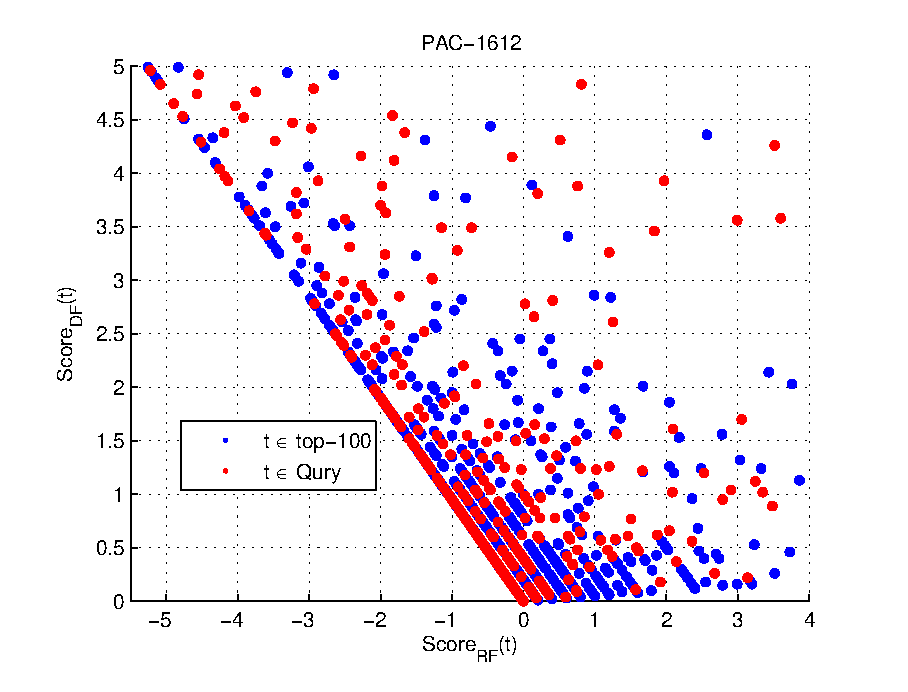
\includegraphics[width=9cm]{figs/qterm_rf_df.eps}} \hspace*{0.1cm}\\[1ex]% 
 %\subfigure[IPC Title words vs. Document Frequent terms.\label{fig:scatter_combined_b}]{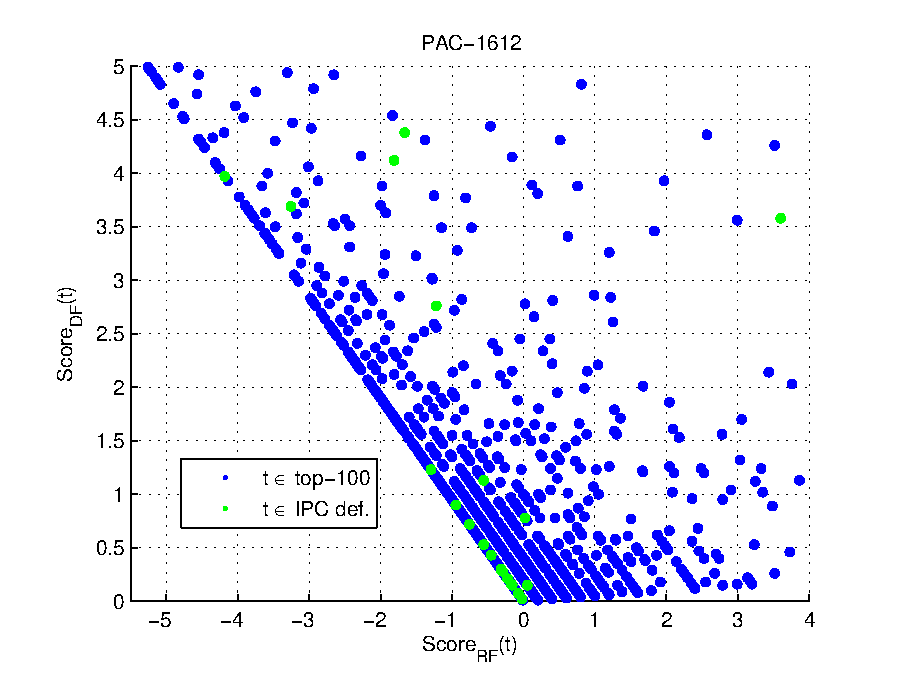
\includegraphics[width=7cm]{figs/ipcdef-rf-df.eps}} 
\subfigure[Query terms ($t \in Query \; \bigwedge \; QTF(t)>5$) versus Document Frequent terms\label{fig:scatter_combined_b}]{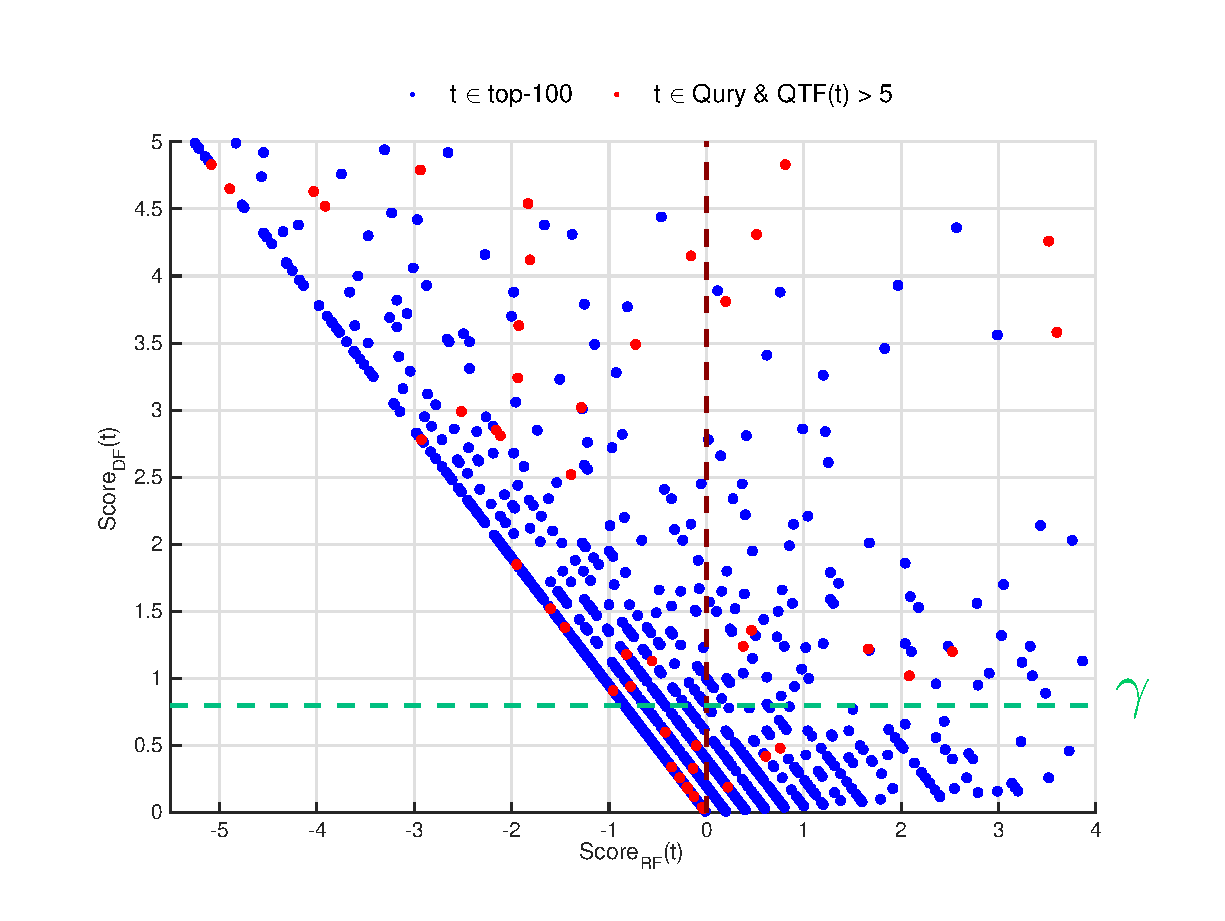
\includegraphics[width=9cm]{figs/df-rf-tauline.eps}}

\par\end{centering}

\protect\caption{Anecdotal example for simple query reduction approaches. Blue points are all terms in a vocabulary set made of top-100 retrieved documents and red points are terms in the Patent Query.}
\label{fig:scatter_combined}
\end{figure}
%%%%%%%%%%%%%%%%%%%%%%%%%%%%%%%%%%%%%%%%%%%%%%%%%%%%%%%%%%%%%%
\subsubsection{Query Reduction Using Pseudo Relevance Feedback}
% TODO: Must be consistent in either pruning or removing terms --- results should ideally converge to the baseline at 0.
% TODO: Should do simplest comparisons first and not combine pruning approaches.  Even better: evaluate methods mentioned in related work.
% TODO: What is an IPC title?  I don't know that this is... was it discussed?
Pseudo Relevance Feedback ($\mathit{PRF}$) is an automated process without user interaction which assumes the top k ranked documents are relevant and the others are irrelevant~\citep{Baeza-Yates2011}. We use $\mathit{PRF}$ to select query terms~\cite{maxwell2013compact} the same as what we did for Oracular Relevance Feedback system (Section~\ref{sec:oraculrquery}). We assume that top 5 retrieved documents are relevant and the rest are irrelevant, then we calculate $\mathit{PRF}$ score based on this assumption:  
%%%%%%%%%%%%%%%%%%%%%%%%%%%%%%%%%%%%%%%%%%%%%%%%%%%%%%%%%%%%%%
\begin{equation}
PRF(t,Q)=Rel(t)-Irr(t) 
 \label{eq:score}
\end{equation}
\vspace*{-2ex}
\begin{displaymath}t\in \lbrace \mbox{terms in top-100 retrieved documents}\rbrace\end{displaymath}
%%%%%%%%%%%%%%%%%%%%%%%%%%%%%%%%%%%%%%%%%%%%%%%%%%%%%%%%%%%%%%  
In the next step, we select the terms in the Patent Query that have the  $\mathit{PRF}$ score higher than the threshold $\tau$ ($PRF(t)>\tau$) to reformulate a reduced query. Figure~\ref{fig:prf} shows slight improvement over the baseline. Compared to the Oracular Term Selection system, this approach did not also help to get any notable improvement over the baseline.
%%%%%%%%%%%%%%%%%%%%%%%%%%%%%%%%%%%%%%%%%%%%%%%%%%%%%%%%%%%%%%
\begin{figure}[t!]
   \centering
   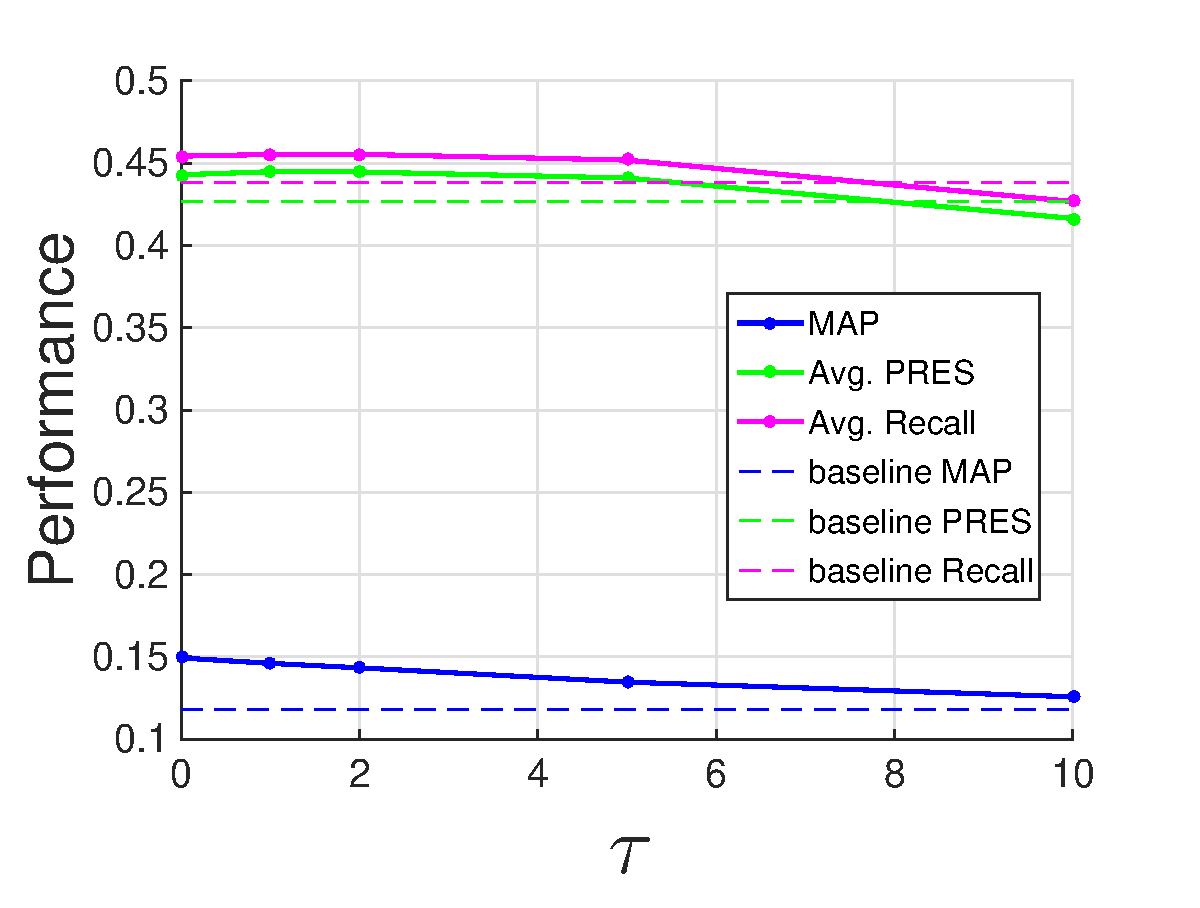
\includegraphics[width=0.50\textwidth,height=55mm]{figs/prf.eps}
   \caption{Query reduction using PRF for various value of the threshold $\tau$.}   
   \label{fig:prf} 
\end{figure}
%%%%%%%%%%%%%%%%%%%%%%%%%%%%%%%%%%%%%%%%%%%%%%%%%%%%%%%%%%%%%%
%%%%%%%%%%%%%%%%%%%%%%%%%%%%%%%%%%%%%%%%%%%%%%%%%%%%%%%%%%%%%%
\begin{figure}[t!]
\begin{centering}
\subfigure[$\tau=0$\label{fig:rf_prf_a}]{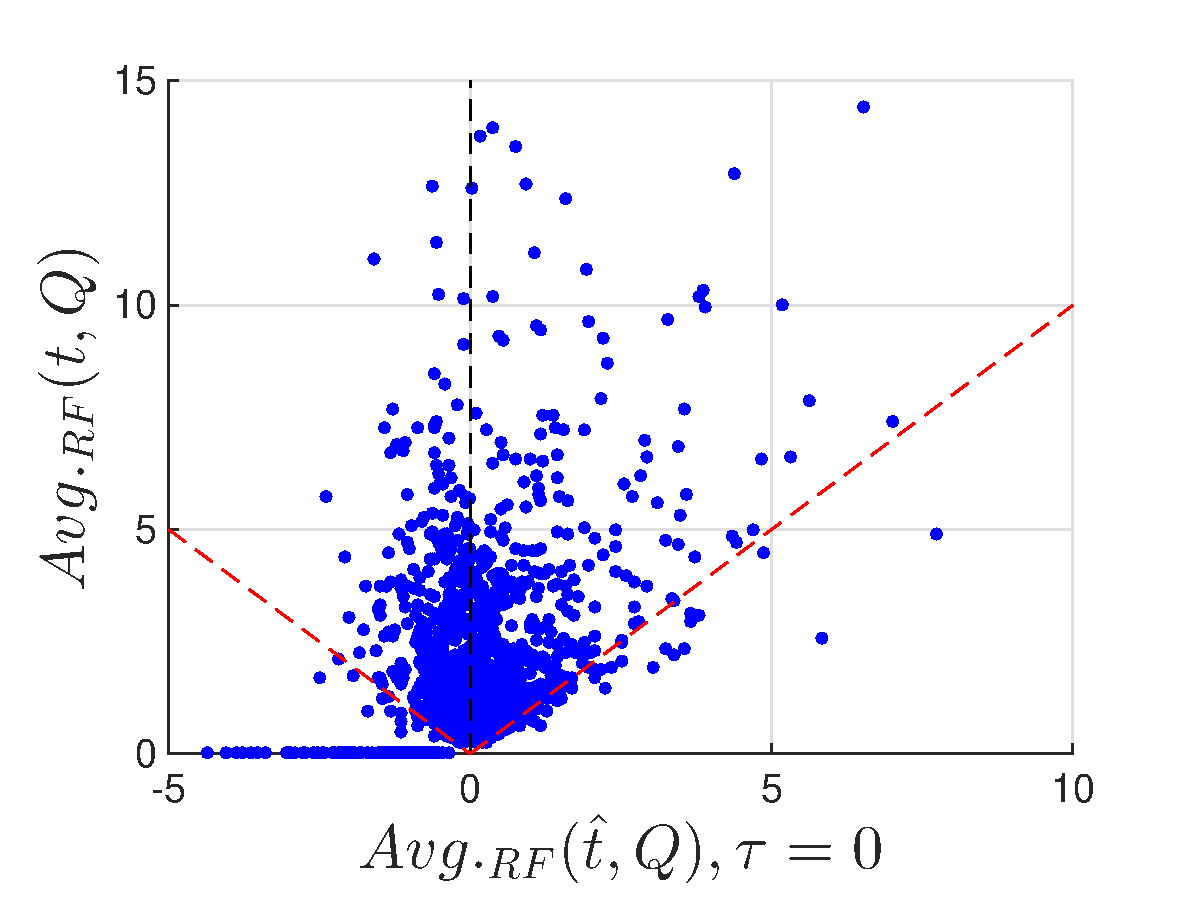
\includegraphics[width=7cm]{figs/scoretscorethat-tau0.eps}} \hspace*{0.1cm}
 \subfigure[$\tau=1$\label{fig:rf_prf_b}]{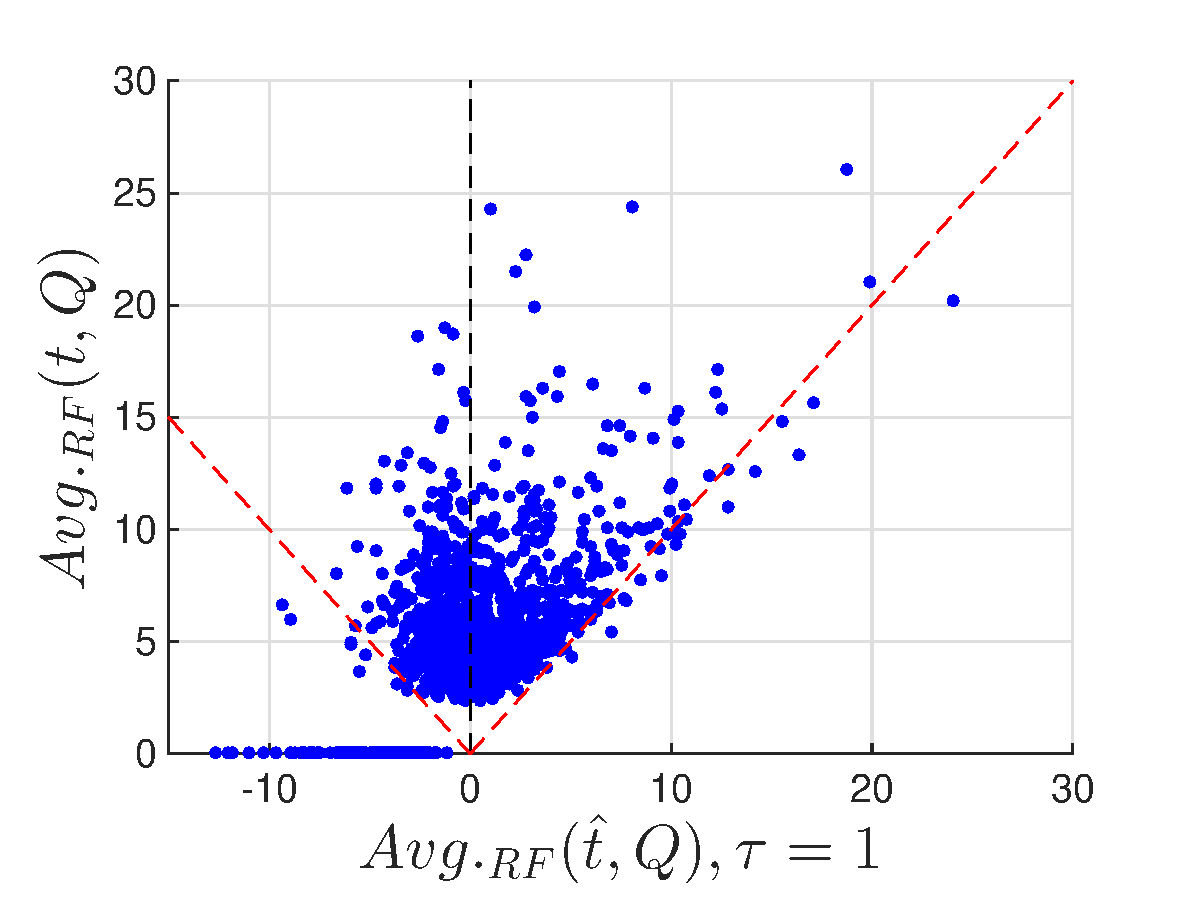
\includegraphics[width=7cm]{figs/scoretscorethat-tau1.eps}} \\[-1ex]% 
\subfigure[$\tau=10$\label{fig:rf_prf_c}]{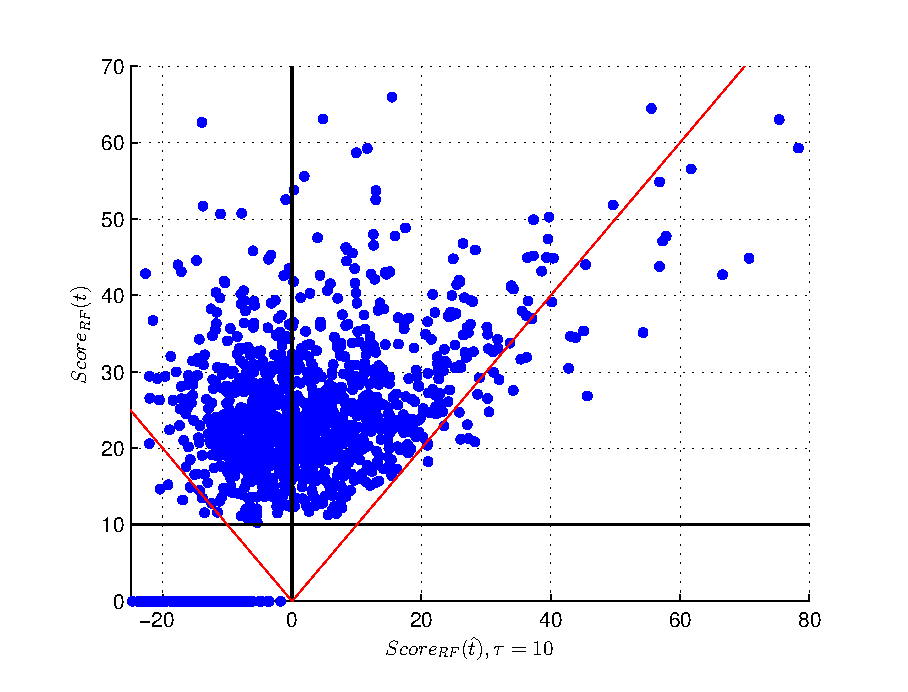
\includegraphics[width=7cm]{figs/scoretscorethat-tau10.eps}}

\par\end{centering}

\protect\caption{Comparing $\mathit{RF}$ score of top Relevance Feedback terms and Pseudo Relevance Feedback terms for different values of the threshold $\tau$.}
\label{fig:rf_prf}
\end{figure}
%%%%%%%%%%%%%%%%%%%%%%%%%%%%%%%%%%%%%%%%%%%%%%%%%%%%%%%%%%%%%%

We analyse why the term selection technique using Pseudo Relevance Feedback fails to approximate the Oracular Patent Query in the following experiment.  
We seek for a pattern between top Relevance Feedback terms and top Pseudo Relevance Feedback terms. For this purpose, we calculate the average $\mathit{RF}$ score of both terms with top  $\mathit{RF}$ score and terms with top $\mathit{PRF}$ score for each query as follows:
%%%%%%%%%%%%%%%%%%%%%%%%%%%%%%%%%%%%%%%%%%%%%%%%%%%%%%%%%%%%
\begin{equation}
Avg_{RF}(t, Q) = \frac{1}{|t|}\sum {RF}(t, Q), \;\;\;\; t\in \{t | RF(t, Q)>\tau\}
\end{equation}
%\begin{displaymath}t\in \{t | RF(t)>\tau\}\end{displaymath}
%%%%%%%%%%%%%%%%%%%%%%%%%%%%%%%%%%%%%%%%%%%%%%%%%%%%%%%%%%%%
\begin{equation}
Avg_{RF}(\hat{t}, Q) = \frac{1}{|\hat{t}|}\sum {RF}(\hat{t}, Q), \;\;\;\; \hat{t}\in \{\hat{t} | PRF(\hat{t}, Q)>\tau\} 
\end{equation}
%\begin{displaymath}\hat{t}\in \{\hat{t} | PRF(\hat{t})>\tau\}\end{displaymath}
%%%%%%%%%%%%%%%%%%%%%%%%%%%%%%%%%%%%%%%%%%%%%%%%%%%%%%%%%%%%

where $Avg_{RF}(t, Q)$ is the average  $\mathit{RF}$ score for top  $\mathit{RF}$-scored terms ($RF(t, Q)>\tau$), $Avg_{RF}(\hat{t}, Q)$ is the average  $\mathit{RF}$ score for top  $\mathit{PRF}$-scored terms ($PRF(\hat{t}, Q)>\tau$), $\tau$ is a threshold for the score to select terms, $t$ is a symbol for terms with high RF score, $\hat{t}$ is a symbol for terms with high $\mathit{PRF}$ score.

Figure~\ref{fig:rf_prf} shows a scatter plot of average $\mathit{RF}$ score for top Relevance Feedback terms and top Pseudo Relevance Feedback terms. First, we observe that almost the RF score of top Relevance Feedback terms is lower than the RF score of top Pseudo Relevance Feedback terms for almost all queries ($ Avg_{RF}(t, Q) > Avg_{RF}(\hat{t}, Q)$). We can also see that for about half of the queries, $Avg_{RF}(\hat{t}, Q)$ is negative, which indicates we are selecting Noisy Terms by their Pseudo Relevance Feedback score rather than Useful Terms. Second, we can find a very slight positive correlation toward selecting positive terms by Pseudo Relevance Feedback, which is the reason that we could get a slight improvement.  

As the last experiment for the automated query reduction, we illustrate why four proposed query reduction approaches failed to approximate the Oracular Patent Query using an anecdotal example of a sample query about an invention related to ``emulsifier''. 
Figure \ref{fig:anecdotal} shows the raw abstract of the invention, and terms and their associated $\mathit{RF}$ scores for each approach. 
Terms are chosen based on the scores for each approach as follows: 
\begin{displaymath}\{t| DF(t)/QTF(t)/PRF(t)>10\}\end{displaymath}
%$\{t| DF(t)/QTF(t)/PRF(t)>10\}$.
For the IPC title terms, all terms appearing in IPC title are displayed since they do not have any score.   
It can be seen that the four methods fail clearly to discriminate between Useful Terms and Noisy Terms. As one example, important stemmed terms like ``enzym'' and ``starch'' have been removed by Document Frequent pruning approach, which hurts query quality.  As another example, retaining IPC code title terms yields more Noisy Terms than Useful Terms (19 out of 32, and few of them with a very negative score like ``amylos'' or ``saccharid''). This can justify slight improvement in performance when we prune terms in IPC title. Overall, all methods may retain highly negative terms and results from Section~\ref{sec:OracularQueryFormulation} showed that the inclusion of even slightly negative terms can significantly hurt the performance.
%In summary, we failed in approximating the Oracular Patent Query with any of four proposed Query reduction techniques.      
%%%%%%%%%%%%%%%%%%%%%%%%%%%%%%%%%%%%%%%%%%%%%%%%%%%%%%%%%%%%
\begin{figure}[htpb]
%\begin{figure}[t!]
\begin{framed}
\vspace*{-2ex}
  \centering
    %\lstinputlisting[frame=single, basicstyle=\scriptsize\ttfamily , linewidth=\columnwidth,breaklines=true]{code/anecdotale.tex}\vspace*{-2ex}
 \begin{lstlisting}[basicstyle=\small\ttfamily , linewidth=\columnwidth,breaklines=true, language=TeX] 
PAC-1293

Abstract: The invention relates to an emulsifier, a method for 
preparing said emulsifier, and to its use in various applications
, primarily food and cosmetic applications. The invention also 
relates to the use of said emulsifier for the creation of an 
elastic, gelled foam. An emulsifier according to the invention is 
based on a starch which is enzymatically converted, using a 
specific type of enzyme, and modified in a specific 
esterification reaction.

(1) DF Terms: <@\textcolor{blue}{starch:14.64}@>, <@\textcolor{blue}{enzym:29.49}@>, <@\textcolor{red}{amylos:-20.15}@>, 
<@\textcolor{blue}{oil:8.63}@>, <@\textcolor{red}{dispers:-8.66}@>, <@\textcolor{red}{ph:-4.55}@>, <@\textcolor{red}{dry:-6.21}@>, <@\textcolor{red}{heat:-2.26}@>, 
<@\textcolor{red}{product:-5.48}@>, <@\textcolor{red}{slurri:-11.48}@>, <@\textcolor{blue}{viscos:7.77}@>, <@\textcolor{red}{composit:-4.49}@>, 
<@\textcolor{red}{reaction:-1.97}@>, <@\textcolor{red}{food:-11.94}@>, <@\textcolor{blue}{agent:5.19}@>, <@\textcolor{red}{debranch:-10.58}@>, 
<@\textcolor{red}{reduc:-6.37}@>, <@\textcolor{red}{fat:-12.83}@>, <@\textcolor{red}{prepar:-0.82}@>, <@\textcolor{red}{hour:-5.42}@>, 
<@\textcolor{blue}{waxi:19.41}@>, <@\textcolor{blue}{deriv:11.97}@>, <@\textcolor{red}{content:-3.38}@>, <@\textcolor{blue}{aqueou:0.38}@>, 
<@\textcolor{red}{saccharid:-11.95}@>, <@\textcolor{red}{ml:-0.79}@>, <@\textcolor{red}{cook:-10.04}@>, <@\textcolor{blue}{modifi:5.65}@>, 
<@\textcolor{blue}{solid:5.50}@>, <@\textcolor{blue}{sampl:6.27}@>, <@\textcolor{blue}{mix:2.48}@>, <@\textcolor{red}{minut:-1.68}@>, <@\textcolor{red}{dri:-0.91}@>, 
<@\textcolor{red}{gel:-9.85}@>, <@\textcolor{blue}{activ:5.98}@>, <@\textcolor{red}{corn:-5.27}@>, <@\textcolor{blue}{alpha:12}@>, <@\textcolor{red}{sprai:-2.74}@> 

(2) QTF Terms: <@\textcolor{blue}{starch:14.64}@>, <@\textcolor{blue}{emulsifi:6.72}@>, <@\textcolor{red}{succin:-3.46}@>, 
<@\textcolor{blue}{enzym:29.49}@>, <@\textcolor{blue}{emuls:12.66}@>, <@\textcolor{blue}{hydrophob:5.45}@>, <@\textcolor{red}{anhydrid:-5.47}@>, 
<@\textcolor{red}{reaction:-1.97}@>, <@\textcolor{red}{octenyl:-0.66}@>, <@\textcolor{blue}{stabil:3.64}@>, <@\textcolor{blue}{alkenyl:0.06}@>, 
<@\textcolor{blue}{reagent:1.17}@>, <@\textcolor{blue}{carbon:0.12}@>, <@\textcolor{blue}{potato:3.74}@>, <@\textcolor{red}{alkyl:-0.33}@>, 
<@\textcolor{red}{wt:-4.57}@>, <@\textcolor{blue}{ether:1.96}@>, <@\textcolor{red}{enzymat:-3.45}@>, <@\textcolor{blue}{convers:10.44}@>, 
<@\textcolor{red}{chain:-5.53}@>, <@\textcolor{blue}{atom:0.03}@>, <@\textcolor{red}{ph:-4.55}@>, <@\textcolor{red}{treat:-0.89}@>, 
<@\textcolor{red}{ammonium:-1.96}@>, <@\textcolor{red}{food:-11.94}@>, <@\textcolor{red}{amylos:-20.15}@>, 
<@\textcolor{red}{glucanotransferas:-0.86}@>, <@\textcolor{red}{glycidyl:-0.40}@>, <@\textcolor{red}{glycosyl:-0.02}@>, 
<@\textcolor{red}{dry:-6.21}@>, <@\textcolor{blue}{deriv:11.97}@>, <@\textcolor{blue}{transferas:0.89}@>, <@\textcolor{red}{foam:-0.49}@>, 

(3) IPC title Terms:<@\textcolor{blue}{cosmet:3.77}@>, <@\textcolor{blue}{toilet:0.18}@>, <@\textcolor{red}{prepar:-0.82}@>, 
<@\textcolor{blue}{case:0.47}@>, <@\textcolor{red}{accessori:-0.01}@>, <@\textcolor{red}{store:-0.37}@>, <@\textcolor{blue}{handl:0.07}@>, 
<@\textcolor{red}{pasti:-0.17}@>, <@\textcolor{red}{substanc:-1.21}@>, <@\textcolor{red}{fibrou:-0.01}@>, <@\textcolor{red}{pulp:-1.28}@>, 
<@\textcolor{red}{constitut:-0.06}@>, <@\textcolor{blue}{paper:1.26}@>, <@\textcolor{red}{impregn:-0.11}@>, <@\textcolor{blue}{emulsifi:6.72}@>, 
<@\textcolor{red}{wet:-0.28}@>, <@\textcolor{red}{dispers:-8.66}@>, <@\textcolor{red}{foam:-0.49}@>, <@\textcolor{red}{produc:-0.57}@>, 
<@\textcolor{blue}{agent:5.19}@>, <@\textcolor{blue}{relev:0.18}@>, <@\textcolor{blue}{class:0.053}@>, <@\textcolor{red}{lubric:-0.38}@>, 
<@\textcolor{blue}{emuls:12.66}@>, <@\textcolor{red}{fuel:-0.011}@>, <@\textcolor{blue}{deriv:11.97}@>, <@\textcolor{blue}{starch:14.64}@>, 
<@\textcolor{red}{amylos:-20.15}@>, <@\textcolor{red}{compound:-0.63}@>, <@\textcolor{red}{saccharid:-11.95}@>, 
<@\textcolor{blue}{radic:1.03}@>, <@\textcolor{red}{acid:-3.19}@> 

(4) PRF Terms: <@\textcolor{blue}{starch:14.64}@>, <@\textcolor{blue}{encapsul:17.50}@>, <@\textcolor{red}{chees:-4.22}@>, 
<@\textcolor{blue}{oil:8.63}@>, <@\textcolor{blue}{hydrophob:5.45}@>, <@\textcolor{blue}{agent:5.19}@>, <@\textcolor{red}{casein:-2.19}@>, 
<@\textcolor{blue}{degrad:17.13}@>, <@\textcolor{blue}{deriv:11.97}@>, <@\textcolor{blue}{tablet:5.30}@>, <@\textcolor{red}{debranch:-10.58}@>, 
<@\textcolor{red}{imit:-1.13}@>, <@\textcolor{blue}{viscos:7.77}@>, <@\textcolor{blue}{oxid:5.97}@>, <@\textcolor{blue}{activ:5.98}@>, <@\textcolor{blue}{osa:9.32}@>, 
<@\textcolor{blue}{funnel:2.68}@>, <@\textcolor{blue}{amylas:26.06}@>, <@\textcolor{red}{amylopectin:-7.14}@>, <@\textcolor{blue}{maiz:20.61}@>, 
<@\textcolor{red}{blend:-3.17}@>, <@\textcolor{blue}{waxi:19.41}@>, <@\textcolor{blue}{convert:31.81}@>, 

 \end{lstlisting} 
 \vspace*{-2ex}
\end{framed}
 \vspace*{-2ex}
  \caption{Four query reduction approaches on a sample query.  Top
    terms retained by each method are shown.  Numerical oracular
    scores $\mathit{RF}(t,Q)$ are provided indicating whether the term
    was useful (blue/positive) or noisy (red/negative).}
  \label{fig:anecdotal}  
\end{figure}
\FloatBarrier
%%%%%%%%%%%%%%%%%%%%%%%%%%%%%%%%%%%%%%%%%%%%%%%%%%%%%%%%%%%%
%\newpage
\subsection{Semi-automated Interactive Reduction}
\label{sec:SemiAutomatedInteractiveReduction}
Our sample analysis of specific queries and terms selected via our oracular
approach suggests that automated methods fall far short of optimal term selection.
This leads us to explore another approach of approximating the oracular query
derived from relevance judgements by using a subset of relevance judgements
through interactive methods.  Specifically, to minimize the need for user interaction,
in this section we analyse the performance of an oracular query derived from
only the first relevant document identified in the search results.
%\begin{comment}
%All our attempts to improve the system effectiveness without accessing the relevance feedback were quite in vein because the features we recognized were tightly the combination of the useful words and noisy words and the system performance is too sensitive to the existence of a noisy word or the absence of the useful terms. So, we decided to apply much more realistic approach in which feedback terms are extracted only from the first ranked relevant document retrieved. 
%\end{comment}
Using this approach, table \ref{tab:firstrel} shows that we can double the MAP in comparison to our baseline and also outperform the PATATRAS system.

Furthermore, to establish the minimal interaction required by this
approach, Figure \ref{fig:FirstTPRankHisto} indicates that the
baseline methods return a relevant patent approximately 80\% of the
time in the first 10 results and 90\% of the time in the first 20
results.  Hence, such an interactive approach requires relatively low
user effort while achieving state-of-the-art performance.
%%%%%%%%%%%%%%%%%%%%%%%%%%%%%%%%%%%%%%%%%%%%%%%%%%%%%%%%%%%%%%%%
\begin{table}[t!]
  \begin{center}
   \caption{System performance using minimal relevance feedback. $\tau$ is RF score threshold, and $k$ indicates the number of first relevant retrieved patents.}\vspace{3mm}
  \input table/partialRFtermselect1.tex   
  \label{tab:firstrel}
  \end{center}  
\end{table}
%\FloatBarrier
%%%%%%%%%%%%%%%%%%%%%%%%%%%%%%%%%%%%%%%%%%%%%%%%%%%%%%%%%%%%%%%%
%%%%%%%%%%%%%%%%%%%%%%%%%%%%%%%%%%%%%%%%%%%%%%%%%%%%%%%%%%%%%%%%
\begin{figure}[t!]
\begin{centering}
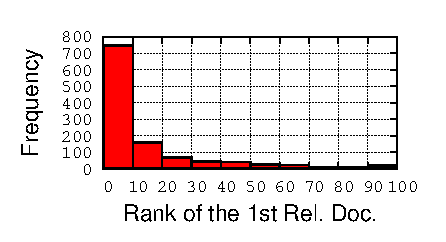
\includegraphics[width=6.5cm, height=3.5cm]{figs/1stRank}
\par\end{centering}

\protect\caption{The distribution of the first relevant document rank over test queries.}
\label{fig:FirstTPRankHisto}
\end{figure}
%\FloatBarrier
%%%%%%%%%%%%%%%%%%%%%%%%%%%%%%%%%%%%%%%%%%%%%%%%%%%%%%%%%%%%%%%%
%%%%%%%%%%%%%%%%%%%%%%%%%%%%%%%%%%%%%%%%%%%%%%%%%%%%%%%%%%%%%%%%
%%%%%%%%%%%%%%%%%%%%%%%%% SECTION 4 %%%%%%%%%%%%%%%%%%%%%%%%%%
%%%%%%%%%%%%%%%%%%%%%%%%%%%%%%%%%%%%%%%%%%%%%%%%%%%%%%%%%%%%%%
%\section{Summary}

